\documentclass[12pt, a4paper, onecolumn, oneside, final]{report}
\usepackage[latin1]{inputenc}
\usepackage[bahasa]{babel}
\usepackage{amsmath}
\usepackage{amsfonts}
\usepackage{amssymb}
\usepackage{tocloft}
\usepackage[left= 3.5cm,right=3cm,top=3cm,bottom=3cm]{geometry}
\usepackage{indentfirst}
\usepackage{amsmath,amssymb,amsfonts,amsthm}
\usepackage{array}
\usepackage{caption}
\usepackage{wrapfig}
\usepackage{graphicx}
\usepackage{varwidth}
\usepackage{float}
\usepackage{indentfirst}
\usepackage{textcomp}
\usepackage{lmodern}
\usepackage{enumerate}
\usepackage{tabularx}
\usepackage{microtype}
\usepackage[framed]{matlab-prettifier}
\usepackage{inputenc}
\usepackage{tikz}
\usepackage{xcolor,colortbl}
\usepackage{multirow}
\usepackage[normalem]{ulem}
\useunder{\uline}{\ul}{}
\usepackage{lscape}
\usepackage{longtable}
\usepackage{times}
\usepackage{float}
\usepackage{hyperref}
\hypersetup{colorlinks=true,
	linkcolor=black,
	filecolor=black,      
	urlcolor=blue,}
%	pdfpagemode=FullScreen,}
\urlstyle{same}
\usepackage{setspace}
\usepackage{enumitem}
\usepackage[labelsep=period]{caption}
\usepackage{pbsi}
\usepackage[T1]{fontenc}
\usepackage{esint}
\usepackage{lipsum}
\usepackage{multirow}
\usepackage{ragged2e}
\usepackage[justification=centering]{caption}
%%
% Hyphenation untuk Indonesia
%
% @author  Andreas Febrian
% @version 2.02
% @edit by Ichlasul Affan
%
% Tambahkan cara pemenggalan kata-kata yang salah dipenggal secara otomatis
% oleh LaTeX. Jika kata tersebut dapat dipenggal dengan benar, maka tidak
% perlu ditambahkan dalam berkas ini. Tanda pemenggalan kata menggunakan
% tanda '-'; contoh:
% menarik
%   --> pemenggalan: me-na-rik
%


% Silakan ganti ke bahasa Inggris (\selectlanguage{english}) jika Anda merasa terlalu banyak kata bahasa Inggris yang pemenggalannya tidak benar.
\selectlanguage{bahasa}


\hyphenation{
    % alphabhet A
    a-na-li-sa a-tur
    a-pli-ka-si
    % alphabhet B
    ba-ngun-an
    be-be-ra-pa
    ber-ge-rak
    ber-ke-lan-jut-an
    ber-pe-nga-ruh
    % alphabhet C
    ca-ri
    % alphabhet D
    di-da-pat-kan di-sim-pan di-pim-pin de-ngan da-e-rah di-ba-ngun da-pat di-nya-ta-kan
    di-sim-bol-kan di-pi-lih di-li-hat de-fi-ni-si di-de-fi-ni-si-kan di-mi-li-ki
    % alphabhet E
    e-ner-gi eks-klu-sif
    % alphabhet F
    fa-si-li-tas
    % alphabhet G
    ga-bung-an ge-rak
    % alphabhet H
    ha-lang-an
    % alphabhet I
    % alphabhet J
    % alphabhet K
    ke-hi-lang-an
    ku-ning
    kua-li-tas ka-me-ra ke-mung-kin-an ke-se-pa-ham-an
    % alphabhet L
    ling-kung-an
    % alphabhet M
    me-neng-ah
    meng-a-tas-i me-mung-kin-kan me-nge-na-i me-ngi-rim-kan
    meng-u-bah meng-a-dap-ta-si me-nya-ta-kan mo-di-fi-ka-si
    meng-a-tur meng-a-rah-kan mi-lik
    % alphabhet N
    nya-ta non-eks-klu-sif
    % alphabhet O
    % alphabhet P
	pe-nye-rap-an
	pe-ngon-trol
    pe-mo-del-an
    pe-ran  pe-ran-an-nya
    pem-ba-ngun-an pre-si-den pe-me-rin-tah prio-ri-tas peng-am-bil-an
    peng-ga-bung-an pe-nga-was-an pe-ngem-bang-an
    pe-nga-ruh pa-ra-lel-is-me per-hi-tung-an per-ma-sa-lah-an
    pen-ca-ri-an pen-ce-ta-kan peng-struk-tur-an pen-ting pen-ting-nya
    % alphabhet Q
    % alphabhet R
    ran-cang-an
    % alphabhet S
    si-mu-la-si sa-ngat
    % alphabhet T
    te-ngah
    ter-da-pat
    trans-for-ma-si
    % alphabhet U
    % alphabhet V
    va-ri-an va-ri-a-si
    % alphabhet W
    % alphabhet X
    % alphabhet Y
    % alphabhet Z
    % special
}

\usepackage{amsmath,amssymb,amsfonts,amsthm}
\usepackage{apacite}
\let\cite\shortcite %ganti setiap shortcite menjadi cite
\usepackage{regexpatch}

%Modifikasi apacite package
\makeatletter
\xpatchcmd{\@@cite}{\def\BCA##1##2{{\@BAstyle ##1}}}{\def\BCA##1##2{{\@BAstyle ##2}}}{}{}
\makeatother

\AtBeginDocument[apacite-localisation]{%
	\renewcommand{\BOthers}[1]{\emph{et al.}\hbox{}}%		%ganti et al menjadi italic
	\renewcommand{\BOthersPeriod}[1]{\emph{et al.}\hbox{}}%	%ganti et al menjadi italic
	\renewcommand{\BBAA}{dan}	%ganti & menjadi dan
	\renewcommand{\BBAB}{dan} % between authors in in-text citation
	\renewcommand{\BAnd}{dan}  % for ``Ed. \& Trans.'' in ref. list
}
\DeclareHookRule{begindocument}{apacite-localisation}{after}{apacite}

%code
\usepackage{listings}
\usepackage{csquotes}
\usepackage{xcolor}

\definecolor{codegreen}{rgb}{0,0.6,0}
\definecolor{codegray}{rgb}{0.5,0.5,0.5}
\definecolor{codepurple}{rgb}{0.58,0,0.82}
\definecolor{backcolour}{rgb}{0.95,0.95,0.92}

\lstdefinestyle{mystyle}{
	backgroundcolor=\color{backcolour},   
	commentstyle=\color{codegreen},
	keywordstyle=\color{magenta},
	numberstyle=\tiny\color{codegray},
	stringstyle=\color{codepurple},
	basicstyle=\ttfamily\footnotesize,
	breakatwhitespace=false,         
	breaklines=true,                 
	captionpos=b,                    
	keepspaces=true,                 
	numbers=left,                    
	numbersep=5pt,                  
	showspaces=false,                
	showstringspaces=false,
	showtabs=false,                  
	tabsize=2
}

\lstset{style=mystyle}
%

\renewcommand{\chaptername}{BAB}
\usepackage{setspace}

\setcounter{tocdepth}{1}

\definecolor{green}{rgb}{0.1,0.1,0.1}
\newcommand{\done}{\cellcolor{teal}done}  %{0.9}
\newcommand{\hcyan}[1]{{\color{teal} #1}}

\newtheorem{theorem}{Dalil}
\newtheorem{corollary}{Akibat}
\newtheorem{lemma}{Lemma}
\newcommand\at[2]{\left.#1\right|_{#2}}
\theoremstyle{definition}
\newtheorem{definition}{Definisi}{}
\newtheorem{example}{\textsf{Contoh}}

\newenvironment{bukti}[1][Bukti]{\noindent{\it\textit{#1. }}}
{\hspace{\stretch{1}}\rule{.5em}{.5em}}

\DeclareMathOperator{\mo}{mod\,}
\DeclareMathOperator{\ord}{ord}
\DeclareMathOperator{\fpb}{fpb}
\newcommand{\defi}{\overset{\mbox{\tiny{\sf def}}}{=}}
\newcommand{\znz}{\Bbb Z/n\Bbb Z}\newcommand{\zpz}{\Bbb Z/p\Bbb Z}
\numberwithin{equation}{chapter}

\setcounter{tocdepth}{3}
\setcounter{secnumdepth}{3}

\setlength\parindent{12.5mm}

\usepackage{blindtext}
\renewcommand\cftbeforetoctitleskip{-1cm}
 \renewcommand\cftbeforeloftitleskip{-1cm}
 \renewcommand\cftbeforelottitleskip{-1cm}
\renewcommand{\cftdotsep}{1}
\renewcommand{\cftchapleader}{\cftdotfill{\cftsecdotsep}}

\renewcommand{\contentsname}{DAFTAR ISI}
\renewcommand{\cfttoctitlefont}{\hfil\Large\bfseries\MakeUppercase}
\renewcommand{\cftchapfont}{\bfseries}
\renewcommand{\cftchappagefont}{\bfseries}
\renewcommand{\cftchappresnum}{BAB }
\renewcommand{\cftchapnumwidth}{3.7em}

\renewcommand{\cftlottitlefont}{\hfil\large\bfseries\MakeUppercase}
\renewcommand{\cfttabpresnum}{Tabel }
\renewcommand{\cfttabnumwidth}{6em}

\renewcommand{\cftloftitlefont}{\hfil\large\bfseries\MakeUppercase}
\renewcommand{\cftfigpresnum}{Gambar }
\renewcommand{\cftfignumwidth}{6em}
\renewcommand{\figurename}{Gambar}

\makeatletter
\def\ps@myPS{%
    \def\@oddfoot{\null\hfill\thepage}
    \def\@evenfoot{\thepage}%
    \def\@evenhead{\null\hfil\slshape\leftmark}%
    \def\@oddhead{{\slshape\rightmark}}}%
\makeatother

\makeatletter % default is "\newcommand\@chapapp{\chaptername}"
\renewcommand\@chapapp{\textls[40]{\MakeUppercase{\chaptername}}}
\makeatletter

\usepackage{titlesec}
% 1. Judul bab ditengah
\titleformat{\chapter}[display]
 {\normalfont\large\bfseries\centering}
 {\chaptertitlename\ \Roman{chapter}}{0pt}{\large}
% 2. Font section 12pt dan tambah titik section, so 1.1 menjadi 1.1.
\titlespacing{\chapter}{0pt}{50pt}{\baselineskip}
\titleformat{\section}[block] %tambah block untuk menampilkan format angka 
 {\normalfont\fontsize{12}{15}\bfseries}{\thesection.}{1em}{}
% 3. Font subsection 12pt dan tambah titik subsection
 \titleformat{\subsection}[block] %tambah block untuk menampilkan format angka 
 {\normalfont\fontsize{12}{15}\bfseries}{\thesubsection.}{1em}{} 
% 4. Hapus spasi setelah bab
\makeatletter
\def\ttl@mkchap@i#1#2#3#4#5#6#7{%
 \ttl@assign\@tempskipa#3\relax\beforetitleunit
 \vspace{\@tempskipa}%<<<<<< REMOVE THE * AFTER \vspace
 \global\@afterindenttrue
 \ifcase#5 \global\@afterindentfalse\fi
 \ttl@assign\@tempskipb#4\relax\aftertitleunit
 \ttl@topmode{\@tempskipb}{%
 \ttl@select{#6}{#1}{#2}{#7}}%
 \ttl@finmarks % Outside the box!
 \@ifundefined{ttlp@#6}{}{\ttlp@write{#6}}}
 
 \usetikzlibrary{shapes.geometric, arrows}
%Spasi sebelum dan sesudah judul sub bab
%\titlespacing*{\section}
%{0pt}{5.5ex plus 1ex minus .2ex}{4.3ex plus .2ex}
%\titlespacing*{\subsection}
%{0pt}{5.5ex plus 1ex minus .2ex}{4.3ex plus .2ex}

\newcommand{\listappendicesname}{DAFTAR LAMPIRAN}
\newlistof{appendices}{apc}{\listappendicesname}
\newcommand{\appendices}[1]{\addcontentsline{apc}{appendices}{#1}}
\renewcommand\cftbeforeapctitleskip{-1cm}
\renewcommand{\cftapctitlefont}{\hfil\large\bfseries\MakeUppercase}

\newcommand{\newappendix}[1]{\section*{#1}\appendices{#1}}

% Tambah kata ejaan yang salah di Latex 
%=====================================================================
% Hyphenation
\hyphenation{
	alphabhet A 
	alphabhet B ber-sum-ber
	alphabhet C 
	alphabhet D dep-loy-ment di-la-ku-kan
	alphabhet E
	alphabhet F 
	alphabhet G 
	alphabhet H 
	alphabhet I incom-pressi-bi-li-ty
	alphabhet J
	alphabhet K kon-tri-bu-si ke-ce-pa-tan ko-si-nus
	alphabhet L lang-sung
	alphabhet M me-ngin-ves-ti-ga-si me-nen-tu-kan mem-per-ka-ya men-da-sa-ri meng-gu-na-kan mem-pe-ro-leh
	alphabhet N 
	alphabhet O
	alphabhet P pe-ne-li-tian per-pin-da-han per-mu-ka-an pe-ngam-bi-lan per-tim-ba-ngan pre-si-pi-ta-si
	alphabhet Q
	alphabhet R
	alphabhet S stra-ti-fi-ka-si Se-dang-kan
	alphabhet T tem-pe-ra-tur ter-ben-tuk te-ri-ma
	alphabhet U
	alphabhet V va-ria-bi-li-tas va-ria-bel
	alphabhet W 
	alphabhet X
	alphabhet Y
	alphabhet Z
	special}
\makeatletter
\renewcommand*\@pnumwidth{3em}
\makeatother

%=====================================================================
\begin{document}

\tikzstyle{rect} = [draw, rectangle, fill=white!20, text width=25em, text centered, minimum height=2em]%text width=20em/13em
\tikzstyle{elli} = [draw, ellipse, fill=white!20, minimum height=2em]
\tikzstyle{circ} = [draw, circle, fill=white!20, minimum height=2em, inner sep=10pt]
\tikzstyle{diam} = [draw, diamond, fill=white!20, text width=6em, text badly centered, inner sep=0pt]
\tikzstyle{line} = [draw, -latex']
%=====================================================================
\pagenumbering{roman}
%=====================================================================
% Halaman Judul
%\addtocontents{toc}{~\hfill{\it Halaman}\par}
\addtocontents{toc}{\begingroup\protect\setlength{\protect\cftsecindent}{-\leftmargin}}
%\addcontentsline{toc}{section}{\protect\numberline{}Judul}
\addtocontents{toc}{\endgroup}
\begin{spacing}{1}
	\begin{center}
		{\Large\textbf{APLIKASI MODEL NUMERIK TIGA DIMENSI UNTUK SIMULASI HIDRODINAMIKA LAUT}}\\[1.0cm]
	\end{center}
	\vspace*{0.8cm} 
	
	\begin{center}
		
		% harus dalam 16pt Times New Roman
		\large{\textbf{PROPOSAL DISERTASI}}
		\\\vspace*{1.8cm}    
		\normalsize{Diajukan untuk melengkapi tugas-tugas dan \\
			memenuhi syarat-syarat guna pelaksanaan penelitian Disertasi}\\[1.5cm]
		%\vspace*{0.3 cm}    
		%% harus dalam 16pt Times New Roman
		\vspace*{1cm}  
		{\large Oleh:}\\
		\vspace*{1cm}       
		% penulis dan NIM
		\large{\textbf{\underline{MUH. NUR HIDAYAT}}}
		\\\large{\textbf{2108201010005}} 
	\end{center}\vspace*{1cm}   
	
	\begin{figure}[h]
		\centering
		
\includegraphics[width=4cm]{contents/Figures/USK} %logo universitas
	\end{figure}
	\vspace*{1.5cm}   
	
	\begin{center}
		% informasi mengenai fakultas dan program studi
		\textbf{PROGRAM STUDI DOKTOR MATEMATIKA DAN APLIKASI SAINS\\
			PROGRAM PASCASARJANA \\
			UNIVERSITAS SYIAH KUALA\\
			DARUSSALAM, BANDA ACEH\\
			JUNI, 2023}
	\end{center}
	\thispagestyle{empty}
\end{spacing}
%=====================================================================
% Halaman Pengesahan
\pagebreak
\chapter*{LEMBAR PENGESAHAN}
\addtocontents{toc}{\begingroup\protect\setlength{\protect\cftsecindent}{-\leftmargin}}
%\addcontentsline{toc}{section}{\protect\numberline{}Pengesahan}	
\addtocontents{toc}{\endgroup}
\setcounter{page}{2}
\vspace{1.5pc}

\begin{center}
	\normalsize
	\noindent
	\begin{tabular}{l l l}
		Judul Disertasi \verb"  " &: Aplikasi Model Numerik Tiga Dimensi untuk Simulasi \\
		& \; Hidrodinamika Laut \\
		Nama Mahasiswa &: Muh. Nur Hidayat \\
		NPM &: 2209300070026 \\
		Program Studi	&: Doktor Matematika dan Aplikasi Sains\\ 
	\end{tabular} \\
\end{center}

\begin{center}
	\vspace{3cm}
	Menyetujui\\
	Komisi Pembimbing, \\
	Promotor \\
	\vspace{2cm}
	\underline{Prof. Dr. Ir. Syamsul Rizal} \\
	NIP. 196101221987031003
	\vspace{1cm}
	
	\begin{tabular}{l l }
		Ko-Promotor I,\verb"                       " & Ko-Promotor II, \verb"            "\\[2.25cm]
		\underline{Prof. Dr. Marwan Ramli, S.Si.,M.Si.} & \underline{Prof. Dr. Muchlisin Z.A, S.Pi.,M.Sc.}\\
		NIP. 197111251999031003 & NIP. 197109111999031003
	\end{tabular}
\end{center}

\begin{center}
	\vspace{0.5cm}
	Mengetahui\\%[0.5cm]
	
	\vspace{1cm}
	
	\begin{tabular}{l l }
		Ketua Program Studi\verb"                  " & \verb" "Direktur Program Pascasarjana\\
		Doktor Matematika dan Aplikasi Sains, & \verb" "Universitas Syiah Kuala,\\[2.25cm]
		\underline{Prof. Dr.rer.nat. Rinaldi Idroes, S.Si.} & \verb" "\underline{Prof. Dr. Ir. Darusman, M.Sc.}\\
		NIP. 196808251994031003 & \verb" "NIP. 196210091987021001
	\end{tabular}
\end{center}
%\vspace{0.3cm}
%\begin{center}
%	
%\end{center}
%\thispagestyle{empty}

%\input{LPS}
%=====================================================================
% Halaman Bebas Plagiasi
%\pagebreak
%\chapter*{PERNYATAAN BEBAS PLAGIASI}
%\addtocontents{toc}{\begingroup\protect\setlength{\protect\cftsecindent}{-\leftmargin}}
%\addcontentsline{toc}{section}{\protect\numberline{}Pernyataan Bebas Plagiasi}	
%\addtocontents{toc}{\endgroup}
%\begin{spacing}{1.5}
	\pagestyle{empty}
	\begin{center}
		\vskip 1cm
		\lipsum[1-3]
	\end{center}
\end{spacing}
\pagestyle{empty}
%=====================================================================
% Halaman Abstrak
%\pagebreak
%\chapter*{ABSTRAK}
%\addtocontents{toc}{\begingroup\protect\setlength{\protect\cftsecindent}{-\leftmargin}}
%%\addcontentsline{toc}{section}{\protect\numberline{}Abstrak}	
%\addtocontents{toc}{\endgroup}
%\begin{spacing}{1.5}
	\pagestyle{empty}
	\begin{center}
		\vskip 1cm
		\lipsum[1-2]
	\end{center}
\end{spacing}
\pagestyle{empty}
%=====================================================================
% Halaman Kata Pengantar
\pagebreak
\chapter*{KATA PENGANTAR}	
\addtocontents{toc}{~\hfill{Halaman}\par} 
\addtocontents{toc}{\begingroup\protect\setlength{\protect\cftsecindent}{-\leftmargin}}
\addcontentsline{toc}{section}{\protect\numberline{}\textbf{KATA PENGANTAR}}
\addtocontents{toc}{\endgroup}
\begin{spacing}{1.5}
	\pagestyle{empty}
	
	\vskip 1cm
	\par Puji syukur kehadirat Allah SWT yang telah melimpahkan nikmat karunia-Nya sehingga proposal penelitian yang berjudul \textbf{Aplikasi Model Numerik Tiga Dimensi untuk Simulasi Hidrodinamika Laut} dapat terselesaikan dengan baik. Penelitian ini dilakukan untuk memenuhi salah satu syarat dalam memperoleh gelar Doktor pada Program Studi Doktor Matematika dan Aplikasi Sains, Universitas Syiah Kuala.
	\par Penyusunan proposal penelitian ini tidak dapat selesai tanpa bantuan dari tim pembimbing. Oleh karena itu, ucapan terima  kasih disampaikan kepada pihak-pihak tersebut.
	\par Proposal penelitian ini tidak luput dari segala kekurangan, baik dalam hal penulisan maupun pembahasan dari topik penelitian. Oleh sebab itu, diperlukan saran demi penyusunan penelitian yang lebih baik. Semoga penelitian dapat memberi manfaat bagi pembaca untuk melaksanakan penelitian selanjutnya.
	\vskip 1cm  
	\begin{flushright}
		Banda Aceh, 15 Juni 2023
		\vskip 2cm
		Penulis	
	\end{flushright}
\end{spacing}
\pagestyle{empty}
%=====================================================================
% Halaman Ringkasan
\pagebreak
\chapter*{RINGKASAN}
\addtocontents{toc}{\begingroup\protect\setlength{\protect\cftsecindent}{-\leftmargin}}
\addcontentsline{toc}{section}{\protect\numberline{}\textbf{RINGKASAN}}	
\addtocontents{toc}{\endgroup}
\begin{spacing}{1.5}
	\pagestyle{empty}
	\begin{center}
		\vskip 1cm
		\justifying
		Penelitian ini membahas tentang \textit{Indian Ocean Dipole} (IOD), yang merupakan perbedaan suhu permukaan laut antara Samudra Hindia bagian barat tropis dan Samudra Hindia bagian timur tropis. IOD memiliki peran penting dalam sistem iklim global dan dampaknya terhadap musim hujan, pertanian, dan perikanan di wilayah tersebut. Karena meningkatnya emisi gas rumah kaca antropogenik, penelitian ini bertujuan untuk memodelkan parameter oseanografi dan meteorologi yang menggerakkan IOD untuk memahami hubungan antara IOD dan perubahan iklim. Penelitian ini menggunakan aplikasi pemodelan laut untuk menganalisis interaksi antara parameter oseanografi seperti suhu, salinitas, dan arus, serta parameter meteorologi seperti tekanan angin dan laju presipitasi. Tujuannya adalah untuk memberikan wawasan tentang mekanisme yang mendorong IOD dan potensi responsnya terhadap perubahan iklim. Penelitian ini diharapkan dapat berkontribusi pada pemahaman kita tentang interaksi kompleks antara laut dan atmosfer di wilayah Samudra Hindia.
	\end{center}
\end{spacing}
\pagestyle{empty}
%=====================================================================
% Halaman Daftar Isi
\pagebreak
\addtocontents{toc}{\begingroup\protect\setlength{\protect\cftsecindent}{-\leftmargin}}
\addcontentsline{toc}{section}{\protect\numberline{}\textbf{DAFTAR ISI}}	
\addtocontents{toc}{\endgroup}
{\hypersetup{linkcolor=black}
\tableofcontents}

%=====================================================================
% Halaman Daftar Tabel
\pagebreak
\renewcommand{\listtablename}{DAFTAR TABEL}
\addtocontents{toc}{\begingroup\protect\setlength{\protect\cftsecindent}{-\leftmargin}}
\addcontentsline{toc}{section}{\protect\numberline{}\textbf{DAFTAR TABEL}}	
\addtocontents{toc}{\endgroup}
\addtocontents{lot}{~\hfill{Halaman}\par}
{\hypersetup{linkcolor=black}
\listoftables}
%=====================================================================
% Halaman Daftar Gambar
\pagebreak
\renewcommand{\listfigurename}{DAFTAR GAMBAR}
\addtocontents{lof}{~\hfill{Halaman}\par}
\addtocontents{toc}{\begingroup\protect\setlength{\protect\cftsecindent}{-\leftmargin}}
\addcontentsline{toc}{section}{\protect\numberline{}\textbf{DAFTAR GAMBAR}}	
\addtocontents{toc}{\endgroup}
{\hypersetup{linkcolor=black}
\listoffigures}
%=====================================================================
% Halaman Daftar Simbol
%\pagebreak
%\chapter*{DAFTAR SIMBOL}
%\addtocontents{toc}{\begingroup\protect\setlength{\protect\cftsecindent}{-\leftmargin}}
%\addcontentsline{toc}{section}{\protect\numberline{}\textbf{DAFTAR SIMBOL}}	
%\addtocontents{toc}{\endgroup}
%\vspace{1.5pc}
\vspace{1.5pc}
\begin{center}
\begin{tabular}{lp{0.75\textwidth}}

\end{tabular}
\end{center}
%=====================================================================
% Halaman Daftar Lampiran
\pagebreak 
{\hypersetup{linkcolor=black}
\listofappendices}
\addtocontents{apc}{~\hfill{Halaman}\par}
\addtocontents{toc}{\begingroup\protect\setlength{\protect\cftsecindent}{-\leftmargin}}
\addcontentsline{toc}{section}{\protect\numberline{}\textbf{DAFTAR LAMPIRAN}}	
\addtocontents{toc}{\endgroup}
%=====================================================================
% Halaman Persembahan
%\pagebreak
%\chapter*{PERSEMBAHAN}
%\addtocontents{toc}{\begingroup\protect\setlength{\protect\cftsecindent}{-\leftmargin}}
%\addcontentsline{toc}{section}{\protect\numberline{}PERSEMBAHAN}	
%\addtocontents{toc}{\endgroup}
%\begin{spacing}{1.5}
	\pagestyle{empty}
	\begin{center}
		\vskip 1cm
		\lipsum[1-3]
	\end{center}
\end{spacing}
\pagestyle{empty}
%=====================================================================
\newpage
\makeatother
\newpagestyle{chapterpage}{\setfoot{}{}{\thepage}}
\assignpagestyle\chapter{chapterpage}
\setcounter{page}{1}
\pagenumbering{arabic}
\pagestyle{myPS}
\def\thechapter{\Roman{chapter}} 
\def\thesection{\arabic{chapter}.\arabic{section}}
\def\thesubsection{\arabic{chapter}.\arabic{section}.\arabic{subsection}}
\def\theequation{\arabic{chapter}.\arabic{equation}}
\def\thefigure{\arabic{chapter}.\arabic{figure}}
\def\thetable{\arabic{chapter}.\arabic{table}}
%=====================================================================% BAB I
\chapter{PENDAHULUAN}
%\vspace{1.5pc}
\vspace{1.5pc}
\section[Latar Belakang]{Latar Belakang}
\begin{spacing}{1.5}
	Samudera Hindia merupakan salah satu dari tiga samudera terbesar di dunia, dengan volume lautan mencapai sekitar 19.8\% dari total volume lautan di seluruh dunia \cite{Eakins2010}. Karena wilayahnya yang sangat luas, Samudera Hindia memiliki peran penting dalam sistem iklim global dan oleh karena itu sangat penting untuk dapat memprediksi perubahan yang terjadi di dalamnya.
	
	IOD atau \textit{Indian Ocean Dipole} merupakan interaksi anomali antara laut dan atmosfer, yang melibatkan osilasi yang tidak teratur dari temperature permukaan laut (SST) di Samudera Hindia tropis. IOD adalah perbedaan SST antara Samudera Hindia bagian barat tropis ($50^\circ$ E-$70^\circ$ E, $10^\circ$ S-$10^\circ$ N) dan Samudera Hindia bagian timur tropis ($90^\circ$ E-$110^\circ$ E, $10^\circ$ S-$0^\circ$ N) \cite{Shunmugapandi2022,Thushara2020,Sattar2019}. Kekuatan IOD diukur berdasarkan \textit{dipole mode index} (DMI), untuk menghitung perbedaan anomali temperatur permukaan laut antara Samudera Hindia bagian barat tropis dan Samudera Hindia bagian timur tropis \cite{Saji1999}. Kekuatan dan frekuensi kejadian IOD telah terbukti memiliki dampak signifikan pada iklim musim hujan \cite{Qiu2014}, pertanian \cite{Zhang2016}, dan perikanan \cite{Lan2013} di wilayah tersebut. Dengan peningkatan emisi gas rumah kaca antropogenik, kekhawatiran tentang dampak potensial perubahan iklim pada IOD dan pola iklim yang terkait semakin meningkat.
	
	Untuk lebih memahami hubungan antara IOD dan perubahan iklim, sangat penting untuk memodelkan parameter oseanografi dan meteorologi yang menggerakkan IOD. Penelitian ini akan menggunakan aplikasi pemodelan laut untuk mempelajari keterkaitan antara IOD, parameter oseanografi seperti arus laut, temperatur laut, salinitas, MLD, Chl-a, fluks air tawar, dan fluks panas bersih, dan parameter meteorologi seperti tekanan angin dan laju presipitasi. Dengan menganalisis interaksi antara parameter-parameter ini, penelitian ini bertujuan untuk memberikan wawasan tentang mekanisme yang mendorong IOD dan potensi responsnya terhadap perubahan iklim.
	
	Penggunaan aplikasi pemodelan laut semakin penting dalam studi perubahan iklim, karena memungkinkan para peneliti untuk mensimulasikan dan memprediksi perilaku parameter oseanografi dan meteorologi dari waktu ke waktu. Studi tentang pemodelan laut berkaitan dengan pembentukan model dan sifat-sifat sistem di dalamnya. Dalam praktiknya, pembentukan model ini memanfaatkan model numerik dan program komputasi dengan tujuan untuk mengatasi keterbatasan data observasi (\textit{in situ}), juga untuk alasan efektifitas serta efisiensi biaya dan waktu yang digunakan. Penelitian sebelumnya mengembangkan model numerik dengan menggunakan persamaan Navier-Stokes untuk memodelkan sirkulasi arus laut dan menganalisis variabel hidrodinamika laut lainnya. Sebagai contoh, simulasi arus laut di perairan Indonesia akibat gaya pembangkit angin menggunakan model persamaan Navier-Stokes 2 dimensi \cite{Rizal2018,Ikhwan2019,Haditiar2019}. Dalam penelitian lain, model persamaan Navier-Stokes 3 dimensi digunakan untuk mengkaji sirkulasi arus pasang surut baroklinik M2 dan hidrodinamika laut yang berasal dari fenomena El Nino \cite{Rizal2010,Haditiar2020,Ikhwan2021}.
	
	Model-model ini dapat digunakan untuk mempelajari dampak perubahan iklim pada laut dan ekosistem yang terkait, serta untuk mengembangkan strategi mitigasi dan adaptasi terhadap perubahan tersebut. Dalam penelitian ini, model laut akan digunakan secara jangka panjang untuk mempelajari IOD, yang diharapkan dapat berkontribusi pada pemahaman kita tentang interaksi kompleks antara laut dan atmosfer di wilayah Samudera Hindia. 
%	Selain itu, penelitian ini akan mengeksplorasi dampak potensial dari perubahan iklim pada IOD dan pola iklim yang terkait. Dengan menganalisis data iklim historis dan proyeksi, studi ini akan mengevaluasi potensi perubahan frekuensi dan intensitas kejadian IOD dalam berbagai skenario perubahan iklim. Penelitian ini juga akan mengevaluasi dampak potensial dari perubahan ini pada iklim musim hujan dan sektor perikanan di wilayah tersebut.
	
	\section[Rumusan Masalah]{Rumusan Masalah}
	Secara keseluruhan, masalah utama dari penelitian ini adalah menyelidiki hubungan antara IOD, parameter oseanografi, dan meteorologi seperti arus laut, temperatur laut, salinitas, MLD, Chl-a, fluks air tawar, fluks panas bersih, laju presipitasi, dan tekanan angin dengan menggunakan aplikasi pemodelan laut, serta mengevaluasi dampak potensial perubahan pada IOD dan pola iklim yang terkait. Dengan memahami mekanisme yang mendorong IOD dan dampaknya terhadap perubahan iklim, penelitian ini diharapkan akan memberikan kontribusi pada ilmu pengetahuan, yaitu pemahaman tentang interaksi kompleks antara laut dan atmosfer serta memberikan strategi untuk mitigasi dan adaptasi terhadap dampak perubahan iklim di wilayah Samudera Hindia.

	\section[Tujuan Penelitian]{Tujuan Penelitian}
	
	Tujuan umum dari penelitian ini adalah menyelidiki hubungan antara IOD dengan parameter oseanografi dan meteorologi seperti arus laut, temperatur laut, salinitas, MLD, Chl-a, fluks air tawar, fluks panas bersih, laju presipitasi, dan tekanan angin, serta dampaknya terhadap ekosistem laut dengan cara menjawab beberapa tujuan khusus berikut.
	
	\begin{itemize}
		\item Menggambarkan peta IOD, arus laut, temperatur laut, salinitas, MLD, Chl-a, fluks air tawar, fluks panas bersih, laju presipitasi, dan tekanan angin di Samudera Hindia.
		\item Menggambarkan dan menganalisis model musiman untuk parameter-parameter oseanografi dan meteorologi, seperti arus laut, temperatur laut, salinitas, MLD, Chl-a, fluks air tawar, fluks panas bersih, laju presipitasi, dan tekanan angin di Samudera Hindia.
		\item Melakukan analisis korelasi untuk mengukur kekuatan dan arah dari hubungan antara IOD dengan parameter-parameter oseanografi dan meteorologi.
	\end{itemize}
	\section[Urgensi Penelitian]{Urgensi Penelitian}

	Samudera Hindia merupakan rumah bagi populasi biota laut yang besar dan semakin bertumbuh, di mana banyak dari mereka bergantung pada sumber daya maritimnya. IOD telah terbukti memiliki dampak signifikan pada keanekaragaman hayati laut, perikanan, dan masyarakat pesisir, terutama selama peristiwa ekstrem seperti kekeringan \cite{Pan2018} dan siklon \cite{Wahiduzzaman2022}. Frekuensi dan intensitas peristiwa ini semakin meningkat dari hari ke hari karena pengaruh perubahan iklim. Oleh karena itu, penting untuk memahami mekanisme yang mendorong variasi IOD agar dapat mengembangkan strategi adaptasi dan mitigasi yang efektif.
	
	Selain itu, Samudera Hindia adalah pemain utama dalam sistem iklim global, dengan keterkaitan yang kuat dengan Samudera Pasifik dan Samudera Atlantik. Perubahan di Samudera Hindia dapat memiliki dampak signifikan pada pola iklim global, terutama melalui pengaruhnya pada sistem musim hujan yang menyediakan air dan makanan bagi miliaran orang di Asia dan Afrika. Oleh karena itu, memahami interaksi kompleks antara IOD dan parameter-parameter oseanografi dan meteorologi lainnya sangat penting untuk proyeksi dan pengembangan model iklim.
	
	Wilayah Samudera Hindia saat ini mengalami perubahan lingkungan yang cepat akibat aktivitas manusia dan perubahan iklim. Perubahan ini mempengaruhi sifat fisik dan kimia laut, seperti temperatur laut, salinitas, dan ketersediaan nutrisi, yang pada gilirannya mempengaruhi siklus biogeokimia dan ekosistem. IOD adalah salah satu penggerak utama dari perubahan ini, dan memahami korelasinya dengan parameter lain sangat penting untuk memprediksi dan mengurangi dampaknya pada wilayah Samudera Hindia.
	
	Secara keseluruhan, penelitian tentang korelasi antara IOD dan berbagai parameter oseanografi dan meteorologi sangat mendesak untuk dilakukan karena dampak signifikan dari parameter-parameter ini pada wilayah Samudera Hindia, pola iklim global, dan kesejahteraan jutaan orang. Karena perubahan iklim terus mengubah sifat fisik dan kimia laut, memahami korelasi ini kritis untuk mengembangkan strategi adaptasi dan mitigasi yang efektif.
	\section[Manfaat Penelitian]{Manfaat Penelitian}
	
	Manfaat dan kebaruan penelitian tentang IOD terletak pada potensi untuk lebih memahami interaksi kompleks antara berbagai parameter oseanografi dan meteorologi serta dampaknya terhadap wilayah Samudera Hindia. Meskipun beberapa penelitian telah meneliti korelasi antara IOD dengan berbagai parameter oseanografi dan meteorologi, masih banyak yang harus dipelajari tentang mekanisme yang mendorong hubungan ini.
	Selain itu, karena perubahan iklim terus mengubah sifat fisik dan kimia Samudera Hindia, semakin penting untuk memahami bagaimana perubahan ini akan memengaruhi IOD dan sistem ekologi, sosial, dan ekonomi yang terkait. 
	
	Secara khusus, manfaat dari penelitian ini adalah
	\begin{itemize}
		\item Memperoleh peta IOD, arus laut, temperatur laut, salinitas, MLD, Chl-a, fluks air tawar, fluks panas bersih, laju presipitasi, dan tekanan angin di Samudera Hindia.
		\item Peta dan hasil analisis model musiman untuk parameter-parameter oseanografi dan meteorologi, seperti arus laut, temperatur laut, salinitas, MLD, Chl-a, fluks air tawar, fluks panas bersih, laju presipitasi, dan tekanan angin di Samudera Hindia.
		\item Hasil analisis korelasi untuk mengukur kekuatan dan arah dari hubungan antara IOD dengan parameter-parameter oseanografi dan meteorologi.
	\end{itemize}
	
	Adapun target jenis luaran dari penelitian ini dapat dilihat dalam Tabel \ref{tab:luaran}
	% Please add the following required packages to your document preamble:
	% \usepackage{multirow}
	\begin{table}[htp]
		\centering
		\caption{Jenis luaran dan indikator capaian tiap tahun}
		\label{tab:luaran}
		\begin{tabular}{|l|l|lll|}
			\hline
			\multirow{2}{*}{No} & \multirow{2}{*}{Jenis Luaran}                                                                                       & \multicolumn{3}{l|}{Indikator Capaian}                                                                                                                                        \\ \cline{3-5} 
			&                                                                                                                     & \multicolumn{1}{l|}{TS1} & \multicolumn{1}{l|}{TS+1}                                                         & TS+2                                                           \\ \hline
			1                   & \begin{tabular}[c]{@{}l@{}}Artikel ilmiah dimuat di \\ jurnal indeks bereputasi (JIB) \\ internasional\end{tabular} & \multicolumn{1}{l|}{}    & \multicolumn{1}{l|}{\begin{tabular}[c]{@{}l@{}}2 draft/\\ submitted\end{tabular}} & \begin{tabular}[c]{@{}l@{}}2 reviewed/\\ accepted\end{tabular} \\ \hline
			2                   & \begin{tabular}[c]{@{}l@{}}Artikel ilmiah dimuat di \\ prosiding internasional\end{tabular}                         & \multicolumn{1}{l|}{}    & \multicolumn{1}{l|}{\begin{tabular}[c]{@{}l@{}}1 draft/\\ submitted\end{tabular}} & \begin{tabular}[c]{@{}l@{}}1 reviewed/\\ accepted\end{tabular} \\ \hline
			3                   & Disertasi                                                                                                           & \multicolumn{1}{l|}{}    & \multicolumn{1}{l|}{}                                                             & 1                                                              \\ \hline
		\end{tabular}
	\end{table}
%	\section[Sistematika Disertasi]{Sistematika Disertasi}
%
%	Penelitian disertasi ini menggunakan gaya penulisan \textit{working chapter}. Setiap publikasi yang dihasilkan disajikan dalam bentuk bab. Terdapat em
%	Tesis ini tersusun atas 5 bab. Bab pertama menjelaskan pendahuluan tentang latar belakang mengapa penelitian ini dilakukan, background masalah yang mendasari, tujuan penelitian, manfaat penelitian, serta kebaruan dari penelitian. Bab kedua berisikan tinjauan pustaka menyangkut ulasan singkat materi penelitian. Bab ketiga membahas tentang metode penelitian yang dilakukan, data yang yang digunakan, serta diagram alir (\textit{flowchart}) dari penelitian. Bab keempat membahas hasil dan pembahasan penelitian. Terakhir, bab kelima membahas tentang kesimpulan dari penelitian.
	
\end{spacing}
%=====================================================================
% BAB II
\chapter{TINJAUAN PUSTAKA}
%\vspace{1.5pc}
\vspace{1.5pc}
%\section[State of the Art]{State of the Art}
\vspace{-1pc}
\section[Penelitian Terkait IOD]{Penelitian Terkait IOD}
\begin{spacing}{1.5}
	Hasil analisis data observasi selama 40 tahun (1958-1997) menunjukkan fenomena mode dipol di Samudera Hindia. Pola variasi internal dengan anomali \textit{sea surface temperature} (SST) rendah di sekitar Sumatra dan tinggi di sebelah barat Samudera Hindia, disertai dengan angin dan presipitasi. Keterkaitan spasial-temporal antara SST dan angin kuat melalui medan presipitasi dan dinamika laut. Proses interaksi udara-laut ini unik dan terbukti independen dari fenomena osilasi selatan El Nino (ENSO). Penemuan mode dipol ini menjelaskan sekitar 12\% variasi SST di Samudera Hindia, yang juga menyebabkan curah hujan yang parah di Afrika timur dan kekeringan di Indonesia selama tahun-tahun aktifnya \cite{Saji1999}.
	
	\citeA{Liu2023} menunjukkan anomali salinitas positif yang signifikan di lapisan atas Samudera Hindia tropis pusat selama periode tertentu. Pada tahun 2010 dan 2016, pengaruh La Nina dan IOD negatif (nIOD) menyebabkan anomali salinitas positif di Samudera Hindia timur akibat adanya angin barat yang kuat dan arus zona positif. \citeA{Chu2022} mempelajari dinamika variasi antartahunan arus khatulistiwa di Samudera Hindia dan mengukur efek dari mode iklim ENSO dan IOD pada arus. \citeA{Xing2022} mengeksplorasi respons arus laut khatulistiwa selama fase puncak IOD, yang memberikan umpan balik positif laut yang mendukung puncak IOD. \citeA{Zhang2021} meneliti tentang Atlantic Nino dan dampaknya pada iklim regional dan global. Mereka menemukan bahwa curah hujan yang meningkat di sebelah barat Samudra Hindia tropis selama IOD positif (pIOD) melemahkan pertukaran angin timur di atas Samudra Atlantik tropis dan menyebabkan anomali hangat di wilayah pusat dan timur khatulistiwa Atlantik sehingga memicu Atlantik Nino.
	
	\citeA{Polonsky2021} mengkaji fitur pembentukan lapisan kritis di zona ekuator-tropika Samudera Hindia, dan bagaimana hal tersebut terkait dengan terbentuknya IOD. \citeA{Valsala2020} meneliti dampak IOD pada siklus karbon di atas laut dan variasinya di Samudera Hindia, dengan menggunakan pengamatan biogeo kimia dan model sirkulasi biogeo kimia laut global. Mereka menemukan bahwa IOD menyebabkan variasi signifikan dalam pengeluaran CO$_2$ dari laut ke udara di wilayah tenggara tropika Samudera Hindia karena dinamika \textit{upwelling} dan anomali yang bergerak ke barat. \citeA{Zhang2020} membedakan IOD dari pola tripole baru yang baru saja ditemukan, yang memiliki \textit{sea surface temperature anomalies} (SSTA) positif (negatif) di atas wilayah tengah tropika (tenggara dan barat) Samudera Hindia. Studi-studi ini membantu untuk memahami interaksi kompleks antara arus laut, kondisi atmosfer, dan variabilitas iklim di Samudera Hindia.
	
	Terkait dengan SST dan \textit{sea surface salinity} (SSS), \citeA{Akhil2023} menemukan bahwa penyegaran permukaan laut di bagian tenggara Laut Arab (SEAS) selama musim dingin dipicu oleh adveksi horizontal air tawar \textit{Bay of Bengal} (BoB) oleh sirkulasi siklonik di sekitar India selama musim gugur, dan IOD menjadi penggerak utama dari variasi antartahunan SSS di SEAS selama musim dingin. Namun, dampak penyegaran SEAS musim dingin terhadap SST lokal dan awal musim hujan berikutnya lemah. \citeA{Genda2022} menemukan bahwa sebelum pertengahan 1950-an, SST bervariasi dengan IOD, sedangkan ENSO juga mempengaruhi variasi SST setelah pertengahan 1950-an. Variasi SSS tidak menunjukkan hubungan dengan faktor-faktor iklim, mengindikasikan bahwa faktor-faktor pengontrol utama SST dan SSS harus dipertimbangkan secara terpisah. \citeA{Sun2022} meneliti respons asimetris SSS yang signifikan terhadap dua kejadian pIOD dan nIOD di selatan Samudera Hindia tropis. Beberapa studi lain juga menyoroti pentingnya IOD dalam menggerakkan variasi antartahunan SSS, seperti penelitian oleh \citeA{Rathore2020} yang menggunakan komposit musiman selama peristiwa ENSO/IOD untuk memahami variasi dalam transportasi kelembaban dan curah hujan di atas Australia, serta asosiasi mereka dengan variasi SSS. Studi lainnya oleh \citeA{Sun2019} dan \citeA{Zhang2016} mengidentifikasi mode dipol salinitas di Samudera Hindia tropis, yang disebut S-IOD, pola variasi SSS antar tahunan dengan anomali salinitas rendah di bagian tengah khatulistiwa dan salinitas tinggi di sebelah tenggara Samudera Hindia tropis.
	
	Selain itu, terdapat penelitian tentang dampak IOD pada kedalaman lapisan campuran (MLD) di Samudera Hindia, seperti penelitian oleh \citeA{Sadhukhan2021} yang menemukan bahwa peristiwa nIOD berasosiasi dengan MLD yang lebih dalam di BoB sedangkan pIOD menyebabkan MLD yang lebih dangkal. Korelasi parsial menunjukkan bahwa fluks panas bersih (NHF) adalah kontributor utama pendalaman MLD di atas BoB utara, sedangkan tekanan angin mengontrol pendalaman di atas BoB selatan. \citeA{Zhang2022} menunjukkan bahwa selama nIOD, MLD menurun karena daerah anomali evaporasi minus presipitasi negatif. Sebaliknya, selama pIOD, MLD meningkat karena daerah anomali evaporasi minus presipitasi positif. 
	
	\citeA{Sun2019} menyelidiki variasi SSS dan hubungannya dengan dinamika laut di Samudera Hindia tropis selatan barat (SWTIO) terkait dengan peristiwa IOD negatif tahun 2010. Mereka menemukan bahwa sirkulasi laut di Samudera Hindia selatan tropis berkontribusi secara signifikan terhadap anomali SSS selama evolusi peristiwa IOD negatif. Kenaikan gelombang Rossby membuat kedalaman termoklin dan MLD dangkal, membawa air subpermukaan berkepadatan tinggi ke lapisan permukaan dan mendinginkan SST, yang lebih menekan presipitasi lokal untuk memberikan umpan balik positif bagi peningkatan SSS. \citeA{Dandapat2021} menemukan bahwa MLD dangkal selama pIOD pada tahun 2006, sedangkan MLD rata-rata lebih dalam (sekitar 50 m) selama nIOD pada tahun 2010. Fluks panas bersih positif pada antarmuka udara-laut juga memainkan peran dominan dalam pendangkalan MLD pada tahun pIOD, karena radiasi gelombang pendek meningkat dan melebihi efek pendinginan fluks panas laten (LHF) selama periode ini. 
	
	\citeA{Sari2020} menemukan bahwa selama peristiwa pIOD kanonik, konsentrasi chl-a yang tinggi diamati di sekitar Selat Sunda dan sepanjang pantai ujung barat Pulau Jawa di sekitar wilayah Cilacap. Namun, selama peristiwa pIOD Modoki, konsentrasi chl-a lebih tinggi dan lebih terdistribusi luas. Hal ini disebabkan oleh peristiwa \textit{upwelling} yang relatif lemah selama peristiwa pIOD Modoki, yang dikombinasikan dengan ketebalan lapisan penghalang yang tipis dan lapisan campuran yang dalam, sehingga memberikan kondisi yang menguntungkan untuk peningkatan konsentrasi chl-a di wilayah Samudra Hindia tropis tenggara. Sementara itu, \textit{upwelling} yang kuat selama peristiwa pIOD kanonik mencegah peningkatan konsentrasi chl-a karena ditunjukkan oleh kedalaman lapisan isotermal yang dangkal yang dikombinasikan dengan ketebalan lapisan penghalang yang tebal dan lapisan campuran yang dangkal. Di sisi lain, \citeA{Devi2017} menemukan bahwa pIOD menyebabkan konsentrasi chl-a yang rendah (<2 mg/m$^3$) dan produktivitas primer yang rendah di Laut Arab (AS). El Nino menyebabkan proses \textit{downwelling}, yang mengakibatkan konsentrasi chl-a rendah (<1 mg/m$^3$ ) di BoB dan AS. La Nina menyebabkan proses \textit{upwelling}, dan menghasilkan konsentrasi chl-a yang tinggi (>2,0 mg/m$^3$ ) di BoB dan AS. 
	
	\citeA{Mandal2022} dan \citeA{Simanjuntak2022} membahas pengaruh ENSO dan IOD pada variasi chl-a di pesisir selatan Jawa dan pantai selatan Pulau Sunda Kecil (LSI) dan menemukan bahwa chl-a yang intens diamati selama tahun-tahun pIOD, sedangkan konsentrasi chl-a paling sedikit diamati selama tahun-tahun nIOD, sementara \citeA{Luang-on2022} menunjukkan bahwa konsentrasi chl-a di Teluk Thailand bagian atas (uGoT) terkait dengan ENSO, bukan IOD. Pada musim SWM, anomali chl-a berkorelasi dengan curah hujan dan debit sungai selama La Nina/El Nino. Pada musim NEM, anomali chl-a berkorelasi dengan debit sungai dan angin selama La Nina/El Nino. Sedangkan pada musim NOM, anomali chl-a berkorelasi dengan kecepatan angin dan curah hujan tinggi selama El Nino.
	
	\citeA{Setiawan2020} meneliti hubungan antara konsentrasi chl-a, SST, dan tekanan angin permukaan laut di Laut Halmahera (HS) yang dipengaruhi oleh Monsun Australia-Indonesia (AIM), ENSO, dan IOD. Pada skala waktu antar tahunan, tekanan permukaan laut dan tekanan angin koheren dengan fase ENSO dan IOD, dan selama peristiwa El Nino dan pIOD (La Nina dan peristiwa nIOD), tekanan permukaan laut dan tekanan angin sangat meningkat (menurun) di HS. Hal ini mendukung peningkatan (pengurangan) konsentrasi chl-a di wilayah tersebut. Penelitian ini menunjukkan bahwa tekanan permukaan laut dan tekanan angin sangat penting dalam menentukan konsentrasi chl-a di HS.
	
	\citeA{Alsayed2023} menunjukkan bahwa pertukaran air antara Teluk Arab (AG) dan Samudera Hindia melalui Selat Hormuz dapat memainkan peran utama dalam variabilitas musiman kandungan panas laut (OHC) di AG. IOD diketahui memengaruhi sirkulasi dan variabilitas Laut Arab, yang berdekatan dengan AG, dan dapat mempengaruhi fluks panas dan air tawar (FWF) di wilayah tersebut. \citeA{Alam2021}  menyelidiki variabilitas fluks panas laten (LE) dan sensibel (H) antartahunan di Samudera Hindia utara pada musim panas dan menemukan bahwa perubahan posisi dan tekanan \textit{South Asia Low} (SAL) dapat menyebabkan perubahan angin permukaan Samudera Hindia utara, kelembaban, dan suhu, yang pada gilirannya mempengaruhi fluks panas udara-laut.
	
	Secara keseluruhan, dari penelitian-penelitian yang telah disebutkan diatas, kebaruan penelitian tentang IOD terletak pada potensi untuk lebih memahami interaksi yang kompleks antara berbagai parameter dan dampaknya terhadap kawasan Samudera Hindia. Menyelidiki pengaruh skala spasial dan temporal yang berbeda pada korelasi IOD, termasuk perbedaan regional dan tren jangka panjang juga merupakan kebaruan dalam penelitian ini. Sementara beberapa penelitian telah meneliti korelasi antara IOD dan berbagai parameter oseanografi seperti arus laut, temperatur laut, salinitas, MLD, Chl-a, fluks air tawar, dan fluks panas, serta paramater meteorologi seperti laju precipitasi, dan tekanan angin masih banyak yang harus dipelajari tentang mekanisme yang mendorong hubungan ini.
	
\end{spacing}
\vspace{-1pc}
\section[Model Numerik dan Parameter]{Model Numerik dan Parameter}
\begin{spacing}{1.5}
	\par Dalam subbab ini, akan dibahas mengenai persamaan untuk parameter dan deskripsi tentang model numerik yang digunakan dalam penelitian ini.
	\subsection[Arus Laut, Temperatur Laut, dan Salinitas]{Arus Laut, Temperatur Laut, dan Salinitas}
	
	Model sirkulasi laut atau \textit{Ocean General Circulation Models} (OGCM) menggunakan persamaan Navier-Stokes untuk memodelkan fenomena fisis yang terjadi di lautan. Lautan adalah fluida yang dapat dijelaskan dengan baik dengan pendekatan persamaan-persamaan primitif, yaitu persamaan Navier-Stokes serta persamaan keadaan nonlinier yang menggabungkan dua parameter (temperatur dan salinitas) dengan kecepatan fluida, dan mempertimbangkan beberapa asumsi dan hipotesis \shortcite{madec_gurvan_2022_6334656}.
	
	Beberapa asumsi yang digunakan dalam persamaan Navier-Stokes diantaranya asumsi Boussinesq, asumsi hidrostatik, dan asumsi tak termampatkan (\textit{incompressibility}). Misalkan $\rho$ sebagai densitas in situ, $T$ sebagai temperatur potensial, $S$ sebagai salinitas, $p$ sebagai tekanan, $z$ sebagai koordinat vertikal, dan $g$ sebagai percepatan gravitasi. Asumsi yang digunakan dalam persamaan Navier-Stokes dapat dituliskan sebagai berikut.\\
	Asumsi Boussinesq
	\begin{equation}\label{eq:P1}
		\rho = \rho(T,S,p).
	\end{equation}
	Berdasarkan asumsi Boussinesq, pengaruh variasi densitas terhadap sistem diabaikan kecuali kontribusinya terhadap gaya apung.\\
	Asumsi hidrostatik
	\begin{equation}
		\frac{\partial p}{\partial z} = -\rho g.
	\end{equation}
	Berdasarkan asumsi hidrostatik, persamaan momentum vertikal direduksi menjadi persamaan kesetimbangan antara parameter gradien tekanan vertikal dan gaya apung.\\
	Asumsi tak termampatkan
	\begin{equation}
		\nabla \;.\; U =\frac{\partial u}{\partial x} + \frac{\partial v}{\partial y} + \frac{\partial w}{\partial z} = 0.
	\end{equation}	
	Berdasarkan asumsi tak termampatkan, persamaan 3-D divergensi untuk vektor kecepatan $U = (u,v,w)$ (dalam koordinat kartesius $(x,y,z)$) dianggap sama dengan 0.
	
	Selanjutnya misalkan $U = U_h + wk$ ($h$ adalah notasi vektor horizontal lokal di atas bidang $(i,j)$). Persamaan vektor invarian (invarian di bawah transformasi koordinat sehingga dapat diterapkan secara seragam dalam sistem koordinat lengkung ortogonal mana pun) dari persamaan primitif dalam sistem vektor $(i, j, k)$ dapat dituliskan dalam persamaan berikut \shortcite{madec_gurvan_2022_6334656}.\\
	Persamaan kesetimbangan momentum
	\begin{equation}\label{eq:P2}
		\begin{aligned}
			\frac{\partial U_h}{\partial t} = - \left[(\nabla \times U) \times U + \frac{1}{2}\nabla (U^2)\right]_h - f \; k \times U_h - \frac{1}{\rho_o}\nabla_h p + D^U + F^U.
		\end{aligned}
	\end{equation}
	Dalam Persamaan (\ref{eq:P2}) di atas, suku $(\nabla \times U) \times U + \frac{1}{2}\nabla (U^2)$ dapat ditulis sebagai $U\cdot \nabla U$ dan merupakan suku percepatan konvektif dari persamaan momentum. Suku $\nabla_h p$ merupakan gradien tekanan, $f = 2\Omega\; \cdot \;k$ merupakan percepatan Coriolis (dengan $\Omega$ adalah vector kecepatan sudut bumi), $D^U$ merupakan parameterisasi dari fisika skala kecil untuk momentum sedangkan $F^U$ merupakan suku gaya permukaan untuk momentum.\\
	Persamaan konservasi panas dan salinitas
	\begin{equation}\label{eq:P3}
		\begin{aligned}
			\frac{\partial T}{\partial t} &= - \nabla \; . \; (T\;U)  + D^T + F^T \\
			\frac{\partial S}{\partial t} &= - \nabla \; . \; (S\;U)  + D^S + F^S,
		\end{aligned}
	\end{equation}
	dengan operator $\nabla$ sebagai vektor turunan yang diperumum dalam arah $(i,j,k)$, parameter $D^T$ dan $D^S$ merupakan parameterisasi dari fisika skala kecil untuk temperatur dan salinitas sedangkan parameter $F^T$ dan $F^S$ merupakan suku gaya permukaan untuk temperatur dan salinitas. 
	
	\subsection[Klorofil-a dan Kedalaman Lapisan Campuran]{Klorofil-a dan Kedalaman Lapisan Campuran}
	Klorofil-a (chl-a) adalah pigmen fotosintetik utama yang ditemukan pada tanaman, alga, dan bakteri fotosintetik. Di laut, chl-a adalah pigmen yang paling banyak ditemukan pada fitoplankton (mikroorganisme fotosintetik yang membentuk dasar dari rantai makanan laut) dan memainkan peran penting dalam siklus karbon dan oksigen di laut, karena proses fotosintesis yang menghasilkan oksigen terjadi berkat keberadaan pigmen ini. Selain itu, chl-a juga digunakan sebagai indikator kualitas air laut, karena konsentrasinya dapat memberikan petunjuk tentang produktivitas biologis di perairan tersebut. Data chl-a yang digunakan dalam penelitian ini merupakan produk hasil dari model biogeo kimia PISCES \cite{gmd-8-2465-2015} dan merupakan bagian dari model OGCM, NEMO. 
	
	Persamaan untuk biomassa chl-a ($I^{chl}$) (dimana $I$ dapat berupa \textit{Pytoplankton} (P) atau \textit{Diatom} (D)) untuk kedua kelompok fitoplankton adalah diparameterisasi menggunakan model foto-adaptif \citeA{geider1997dynamic}:
	\begin{equation}\label{eq:chl1}
		\begin{aligned}
			\frac{\partial I^{chl}}{\partial t} &= (1-\delta ^I)(12\theta^{chl}_{min}+(\theta^{chl,I}_{max}-\theta^{chl,I}_{min})\rho^{I^{chl}})\mu^I I-m^I \frac{I}{K_m +I}I^chl \\
			&- sh \times w^I II^{chl}-\theta^{chl,I}g^Z(I)Z-\theta^{chl,I}g^M(I)M,
		\end{aligned}
	\end{equation}
	dengan $I$ adalah kelompok fitoplankton dan $\theta^{chl,I}$ adalah rasio klorofil-ke-karbon dari kelas fitoplankton yang dipertimbangkan, 12 mewakili massa molar karbon, $\rho^{I^Chl}$ adalah rasio energi yang terasimilasi terhadap energi yang diserap.
	
	Kedalaman lapisan campuran atau MLD dapat dihitung dengan menggunakan temperatur laut, salinitas, atau densitas laut. MLD yang dihitung dengan temperatur dapat ditemukan pada kedalaman laut dengan temperatur yang relatif konstan. Lapisan campuran terbentuk karena adanya pengaruh angin permukaan, gelombang, dan arus yang menyebabkan pencampuran air pada lapisan atas dan membagikan panas ke seluruh lapisan ini. Di bawah lapisan campuran terdapat perubahan temperatur yang cepat seiring dengan peningkatan kedalaman laut, lapisan ini dikenal sebagai termoklin. MLD dapat diestimasi dari kombinasi variabel ambang batas dari profil densitas dan profil temperatur laut 0.2$^o$C (Pers. \ref{eq:chl2}) \cite{Boyer2004}. 
	Kriteria variabel dalam densitas sesuai dengan variasi temperatur lokal sebesar 0.2$^o$C dari temperatur pada kedalaman 10 meter (Pers. \ref{eq:chl3}). Hasil MLD akhir adalah nilai minimum dari MLD yang dihitung dari kriteria kepadatan dan MLD dari kriteria temperatur. Untuk kedua kriteria, kepadatan dan temperatur, hasil MLD menghasilkan interpolasi linear ke kedalaman di mana ambang batas tercapai.
	\begin{equation}\label{eq:chl2}
		\begin{aligned}
			MLD= \text{Kedalaman dimana }(\sigma_0=\sigma_{0_{10m}}+\Delta \sigma_0)
		\end{aligned}
	\end{equation}
	\begin{equation}\label{eq:chl3}
		\begin{aligned}
			MLD= \text{Kedalaman dimana }(T=T_{10m}+\Delta \pm 0.2^oC),
		\end{aligned}
	\end{equation}
	dengan $\Delta \sigma_0=\sigma_0(\theta_{10m}-0.2^oC,S_{10m},P_0)-\sigma_0(\theta_{10m},S_{10m},P_0)$.
	\subsection[Fluks Panas Bersih dan Fluks Air Tawar]{Fluks Panas Bersih dan Fluks Air Tawar}
	
	Fluks panas bersih atau \textit{net heat flux} (NHF) adalah jumlah panas yang masuk atau keluar dari permukaan laut, yang disebabkan oleh perbedaan antara temperatur air laut dan temperatur udara di atasnya. Jika temperatur udara lebih tinggi dari temperatur air laut, maka NHF akan masuk ke laut. Sebaliknya, jika temperatur udara lebih rendah dari temperatur air laut, maka NHF akan keluar dari laut. NHF dapat dihitung sebagai jumlah dari komponen-komponen berikut \cite{Tomita2021}: 
	\begin{equation}\label{eq:NHF}
		NHF = SWR + LWR + LHF + SHF,
	\end{equation} 
	dengan SWR=\textit{net shortwave radiation}, LWR=\textit{net long wave radiation}, LHF=\textit{surface latent heat flux}, dan SHF=\textit{sensible heat flux}. Dalam penelitian ini, semua aliran panas diasumsikan positif ketika mereka mengarah ke atas, menjauhi permukaan laut ke atmosfer.
	
	Fluks air tawar atau \textit{freshwater flux} (FWF) adalah jumlah air tawar yang masuk atau keluar dari wilayah laut tertentu, termasuk curah hujan, aliran sungai, penguapan, dan es laut. Ketidakseimbangan antara air tawar masuk dan keluar dari wilayah laut dapat berdampak pada sirkulasi laut dan ketersediaan nutrisi bagi organisme laut. FWF dapat dihitung dengan cara sebagai berikut \cite{Tomita2019}:
	\begin{equation}\label{eq:FWF}\\
		\begin{aligned}
		FWF &= EVAP-RAIN, \\
		EVAP &= LHF/{\rho L_e}.
		\end{aligned}
	\end{equation} 
	dengan $EVAP$=evaporasi dan $RAIN$=curah hujan atau presipitasi di atas laut. Sedangkan $\rho$ adalah densitas air laut dan $L_e$ adalah  vaporisasi panas laten dalam air yang didefinisikan sebagai fungsi dari SST.
	\subsection[Laju Presipitasi dan Tekanan Angin]{Laju Presipitasi dan Tekanan Angin}
	Laju presipitasi merupakan tingkat curah hujan yang jatuh ke permukaan laut pada suatu wilayah tertentu. Hal ini dipengaruhi oleh faktor-faktor seperti SST, kelembaban udara, dan angin. Laju presipitasi di laut dapat berpengaruh pada ketersediaan air tawar, salinitas, serta pola sirkulasi dan transportasi massa air di dalam laut. Perhitungan laju presipitasi mengikuti Pers. \ref{eq:FWF}. 
	
	Angin memainkan peran penting dalam mendorong arus permukaan dan juga dalam proses interaksi udara-laut. Sebagian besar proses interaksi udara-laut ditentukan dengan menggunakan tekanan angin (\textit{wind stress}), suatu ukuran transfer momentum yang disebabkan oleh gerakan relatif antara laut dan atmosfer \shortcite{Chacko2022}. Tekanan angin berdasarkan aerodinamis massal (\textit{bulk-aerodynamic}) dirumuskan sebagai,
	\begin{equation}
		\tau = \rho_a C_d U_w^2
	\end{equation}
	dengan $\rho_a$ adalah densitas udara $(1.225 kg/m^3)$, $C_d$ koefisien seret (\textit{dimensionless}) $(\approx 1.3 \times 10^-3)$ dan $U_w$ kecepatan angin.

%	Dalam aplikasinya, persamaan Navier-Stokes tidak hanya digunakan untuk memodelkan laut, tapi juga merambah ke bidang pemodelan cuaca \shortcite{Rohli2021}, aliran air dalam pipa \shortcite{Ouchiha2012} dan aliran udara di sekitar sayap pesawat \shortcite{Tulus2019}. Dalam bentuk persamaan lengkap dan simplifikasi, persamaan ini juga dapat digunakan untuk mendesain kereta api \shortcite{Croquer2020}, pesawat terbang \shortcite{Chau2021}, dan mobil \shortcite{Ambarita2018}. Terdapat juga studi tentang aliran darah \shortcite{Gill2021}, desain stasiun pembangkit listrik \shortcite{Yang2019}, dan analisis polusi udara \shortcite{Issakhov2022}. 
	
\end{spacing}
\vspace{-1pc}
\section[Peta Jalan Penelitian]{Peta Jalan Penelitian}
\begin{spacing}{1.5}
	\textit{Road Map} atau peta jalan penelitian ini dapat dilihat dalam Gambar \ref{fig:RM}
	\begin{figure}[H]
		\centering
		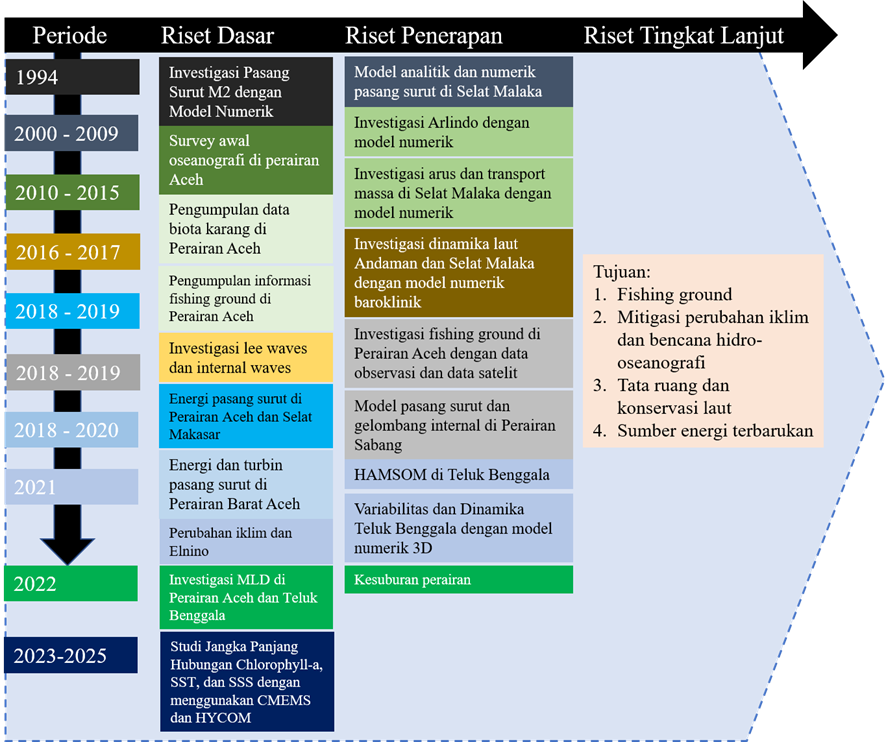
\includegraphics[width=12cm]{contents/Figures/Road_Map}
		\caption{\textit{Road Map} Penelitian}
		\label{fig:RM}
	\end{figure}
	
\end{spacing}
%=====================================================================
% BAB III
\chapter{METODOLOGI PENELITIAN}
\vspace{1.5pc}
\section[Domain dan Data Penelitian]{Domain dan Data Penelitian}
\begin{spacing}{1.5}
	\subsection[Domain Penelitian]{Domain Penelitian}
	Penelitian ini mengkaji hubungan antara IOD, parameter oseanografi (arus laut, temperatur laut, salinitas, MLD, Chl-a, fluks air tawar, fluks panas bersih), dan parameter meteorologi (laju presipitasi dan tekanan angin) di Samudera Hindia dengan koordinat ($0^\circ-24.6^\circ$ N) dan ($78.2^\circ-105^\circ$ E) (lihat Gambar \ref{fig:domain}).

	\subsection[Data Penelitian]{Data Penelitian}
%	\vspace{-1pc}
%		\subsection[NEMO/CMEMS]{NEMO/CMEMS}
%	\par Model NEMO (\textit{Nucleus for European Modelling of the Ocean}) (\href{https://www.nemo-ocean.eu/}{https://www.nemo-ocean.eu/}) adalah model komputasi resolusi tinggi yang terus dikembangkan sejak tahun 2008 oleh konsorsium Eropa yang terdiri dari 5 institusi, yaitu CMCC, CNRS, \textit{Mercator Ocean}, \textit{Met Office}, dan NERC. Model ini digunakan untuk penelitian dan peramalan dalam bidang oseanografi dan klimatologi, dengan tujuan menjadi alat yang fleksibel untuk mempelajari fenomena fisik dan biogeokimia dalam sirkulasi laut, serta interaksinya dengan komponen sistem iklim Bumi, pada skala ruang dan waktu yang berbeda  \shortcite{madec_gurvan_2022_6334656}. Data \textit{output} model NEMO dapat diperoleh dari website CMEMS (\textit{Copernicus Marine Environment Monitoring Service}) \href{https://resources.marine.copernicus.eu/products}{(https://resources.marine.copernicus.eu/products)}. CMEMS merupakan w
%	
%	Data yang tersedia pada website CMEMS dapat dilihat pada Tabel . Resolusi data \textit{output} yang digunakan untuk model ini adalah dx = dy = 5 menit pada bidang horizontal dan 50-lapisan $(k \in [1,50])$ dengan ketebalan berbeda pada bidang vertikal:
%	\begin{equation*}
%		\begin{aligned}
%			z_k = \{0.49, 1.54, 2.65, 3.82, 5.08, 6.44, 7.93, 9.57, 11.40, 13.47, 15.82, 18.50, \\
%			21.60, 25.21, 29.44, 34.43, 40.34, 47.37, 55.76, 65.81, 77.85, 92.33, 109.73, 130.67, \\
%			155.85, 186.12, 222.47, 266.04, 318.13, 380.21, 453.94, 541.089, 643.57, 763.33, \\
%			902.34, 1062.44, 1245.29, 1452.25, 1684.28, 1941.89, 2225.08, 2533.33, 2865.70,  \\
%			3220.82, 3597.03, 3992.48, 4405.22, 4833.29, 5274.78, 5727.92 \} (m). \\
%		\end{aligned}
%	\end{equation*}
%	\subsection[HYCOM]{HYCOM}
%	\par Model HYCOM (\textit{HYbrid Coordinate Ocean Model}) (\href{https://www.hycom.org}{https://www.hycom.org}) adalah salah satu model sirkulasi laut (OGCM) yang menggunakan model numerik tiga dimensi Navier-Stokes dengan input data batimetri dari GEBCO (\textit{General Bathymetric Chart of the Oceans}), data asimilasi hidrografi laut dari NCODA (\textit{Navy Coupled Ocean Data Assimilation}) dan komponen meteorologi dari NCEP (\textit{National Centers for Environmental Prediction}) ataupun NAVGEM (\textit{The NAVy Global Environmental Model}) berupa tekanan angin, kecepatan, fluks panas, tekanan permukaan laut, presipitasi, temperatur laut, dan kelembapan \shortcite{JosephMetzger2013}. 
%	

%	Koordinat vertikal dalam HYCOM adalah isopiknal di lautan terbuka yang terstratifikasi dan memiliki transisi yang mulus dan dinamis serta bergantung terhadap waktu pada medan daerah pesisir yang dangkal dan pada tingkat tekanan tetap di lapisan campuran permukaan atau lautan yang tidak terstratifikasi \shortcite{chassignet2017,Park2013}. Data HYCOM yang digunakan adalah data analisis global arus dan temperatur laut tiga dimensi dengan resolusi spasial 5 menit untuk longitude dan 2.5 menit untuk latitude selama 12 bulan (Januari - Desember) tahun 2021 dan dengan ketebalan bervariasi pada bidang vertikal, yaitu 40-lapisan $(k \in [1,40])$:
%	\begin{equation*}
%		\begin{aligned}
%			z_k = \{0.0, 2.0, 4.0, 6.0, 8.0, 10.0, 12.0, 15.0, 20.0, 25.0, 30.0, 35.0, 40.0, 45.0, 50.0, \\
%			60.0, 70.0,	80.0, 90.0, 100.0, 125.0, 150.0, 200.0, 250.0, 300.0, 350.0, 400.0, 500.0, 600.0,\\
%			700.0, 800.0, 900.0, 1000.0, 1250.0, 1500.0, 2000.0, 2500.0, 3000.0, 4000.0, 5000.0\} (m). \\
%		\end{aligned}
%	\end{equation*}
%	\subsection[J-OFURO3]{J-OFURO3}
%	\subsection[NCEP/NCAR]{NCEP/NCAR}
	Beberapa data yang digunakan dalam penelitian ini adalah data DMI, arus laut, temperatur laut, salinitas, MLD, Chl-a, fluks air tawar, fluks panas bersih, laju presipitasi, dan tekanan angin (lihat Tabel \ref*{tab:data}). Data DMI diperoleh dari \textit{National Oceanic and Atmospheric Administration/Physical Sciences Laboratory} (NOAA/PSL) \cite{Saji2003} sedangkan data arus laut, temperatur laut, salinitas, MLD, dan Chl-a dapat diperoleh dari website penyedia data \textit{Copernicus Marine Environment Monitoring Service} (CMEMS)\cite{Lellouche2018} dan \textit{HYbrid Coordinate Ocean Model} (HYCOM)\cite{Chassignet2007}. Data lainnya adalah fluks air tawar, fluks panas bersih, laju presipitasi, dan tekanan angin yang bersumber dari \textit{National Centers for Environmental Prediction and the National Center for Atmospheric Research reanalysis 1} (NCEP/NCAR) \cite{Kalnay1996} dan J-OFURO3 yang merupakan generasi ketiga dari \textit{Japanese ocean flux data set} yang menggunakan pengamatan penginderaan jarak jauh \cite{Tomita2019}. 
	
%	Hasil yang sangat baik diperoleh dengan membandingkan data temperatur laut 3D (dalam Kelvin) CMEMS dengan data pengamatan \textit{in situ} pada kedalaman 0 hingga 5 m di Samudera Hindia. Hal ini tercermin dari nilai \textit{Root Mean Square} (RMS), untuk perbandingan \textit{in situ thematic centre} (INS TAC), dengan nilai 0.65, dan untuk data \textit{in situ} CORIOLIS, dengan nilai 0.44. Perbandingan data salinitas 3D (dalam satuan salinitas praktis (psu)) dengan data pengamatan \textit{in situ} juga menunjukkan hasil yang sangat baik. Nilai RMS pada kedalaman 0 hingga 5 m untuk data global dan Samudera Hindia masing-masing adalah 0.65 dan 0.204 (Lellouche et al., 2019). Sama halnya dengan perbandingan model CMEMS dan konsentrasi \textit{float} Chl-a (\textit{Biogeochemical-Argo} (BGC-Argo), data pengukuran). Hal ini ditunjukkan oleh koefisien korelasi dan \textit{Root Mean Square Error} (RMSE) masing-masing sebesar 0,81 dan 0,59 (Lamouroux et al., 2019).   
	
	\begin{table}[H]
		\centering
		\caption{Rangkuman data penelitian}
		\label{tab:data}
		\resizebox{\textwidth}{!}{%
		\begin{tabular}{|l|l|l|l|l|}
			\hline
			No & Data               & Periode   & Sumber      & Referensi \\ \hline
			1  & DMI                & 1994-2021 & NOAA/PSL    & \cite{Saji2003}      \\ \hline
			2  & Arus laut               & 1994-2021 & CMEMS/HYCOM & \cite{Lellouche2018,Chassignet2007}      \\ \hline
			3  & Temperatur laut    & 1994-2021 & CMEMS/HYCOM & \cite{Lellouche2018,Chassignet2007}      \\ \hline
			4  & Salinitas          & 1994-2021 & CMEMS/HYCOM & \cite{Lellouche2018,Chassignet2007}     \\ \hline
			5  & MLD                & 1994-2021 & CMEMS       & \cite{Lellouche2018}      \\ \hline
			6  & Chl-a              & 1994-2021 & CMEMS		  & \cite{Lellouche2018}      \\ \hline
			7  & Fluks air tawar    & 1994-2017 & J-OFURO3    & \cite{Tomita2019}      \\ \hline
			8  & Fluks panas bersih & 1994-2017 & J-OFURO3    & \cite{Tomita2019}     \\ \hline
			9  & Laju presipitasi   & 1994-2021 & NCEP/NCAR   & \cite{Kalnay1996}      \\ \hline
			10 & tekanan angin              & 1994-2021 & NCEP/NCAR   & \cite{Kalnay1996}      \\ \hline
		\end{tabular}%
	}
	\end{table}
	\subsection[Pengumpulan Data]{Pengumpulan Data}
	Data dalam Tabel \ref{tab:data} merupakan data yang tersedia secara gratis dan bersifat terbuka. Data ini dapat diunduh secara langsung pada website penyedia data ataupun menggunakan kode skrip. Kode skrip yang digunakan untuk mengunduh data dengan bahasa \textit{Shell script} (terminal Linux) dan Python disajikan dalam Lampiran 1.
	
	\begin{figure}[H]
		\centering
		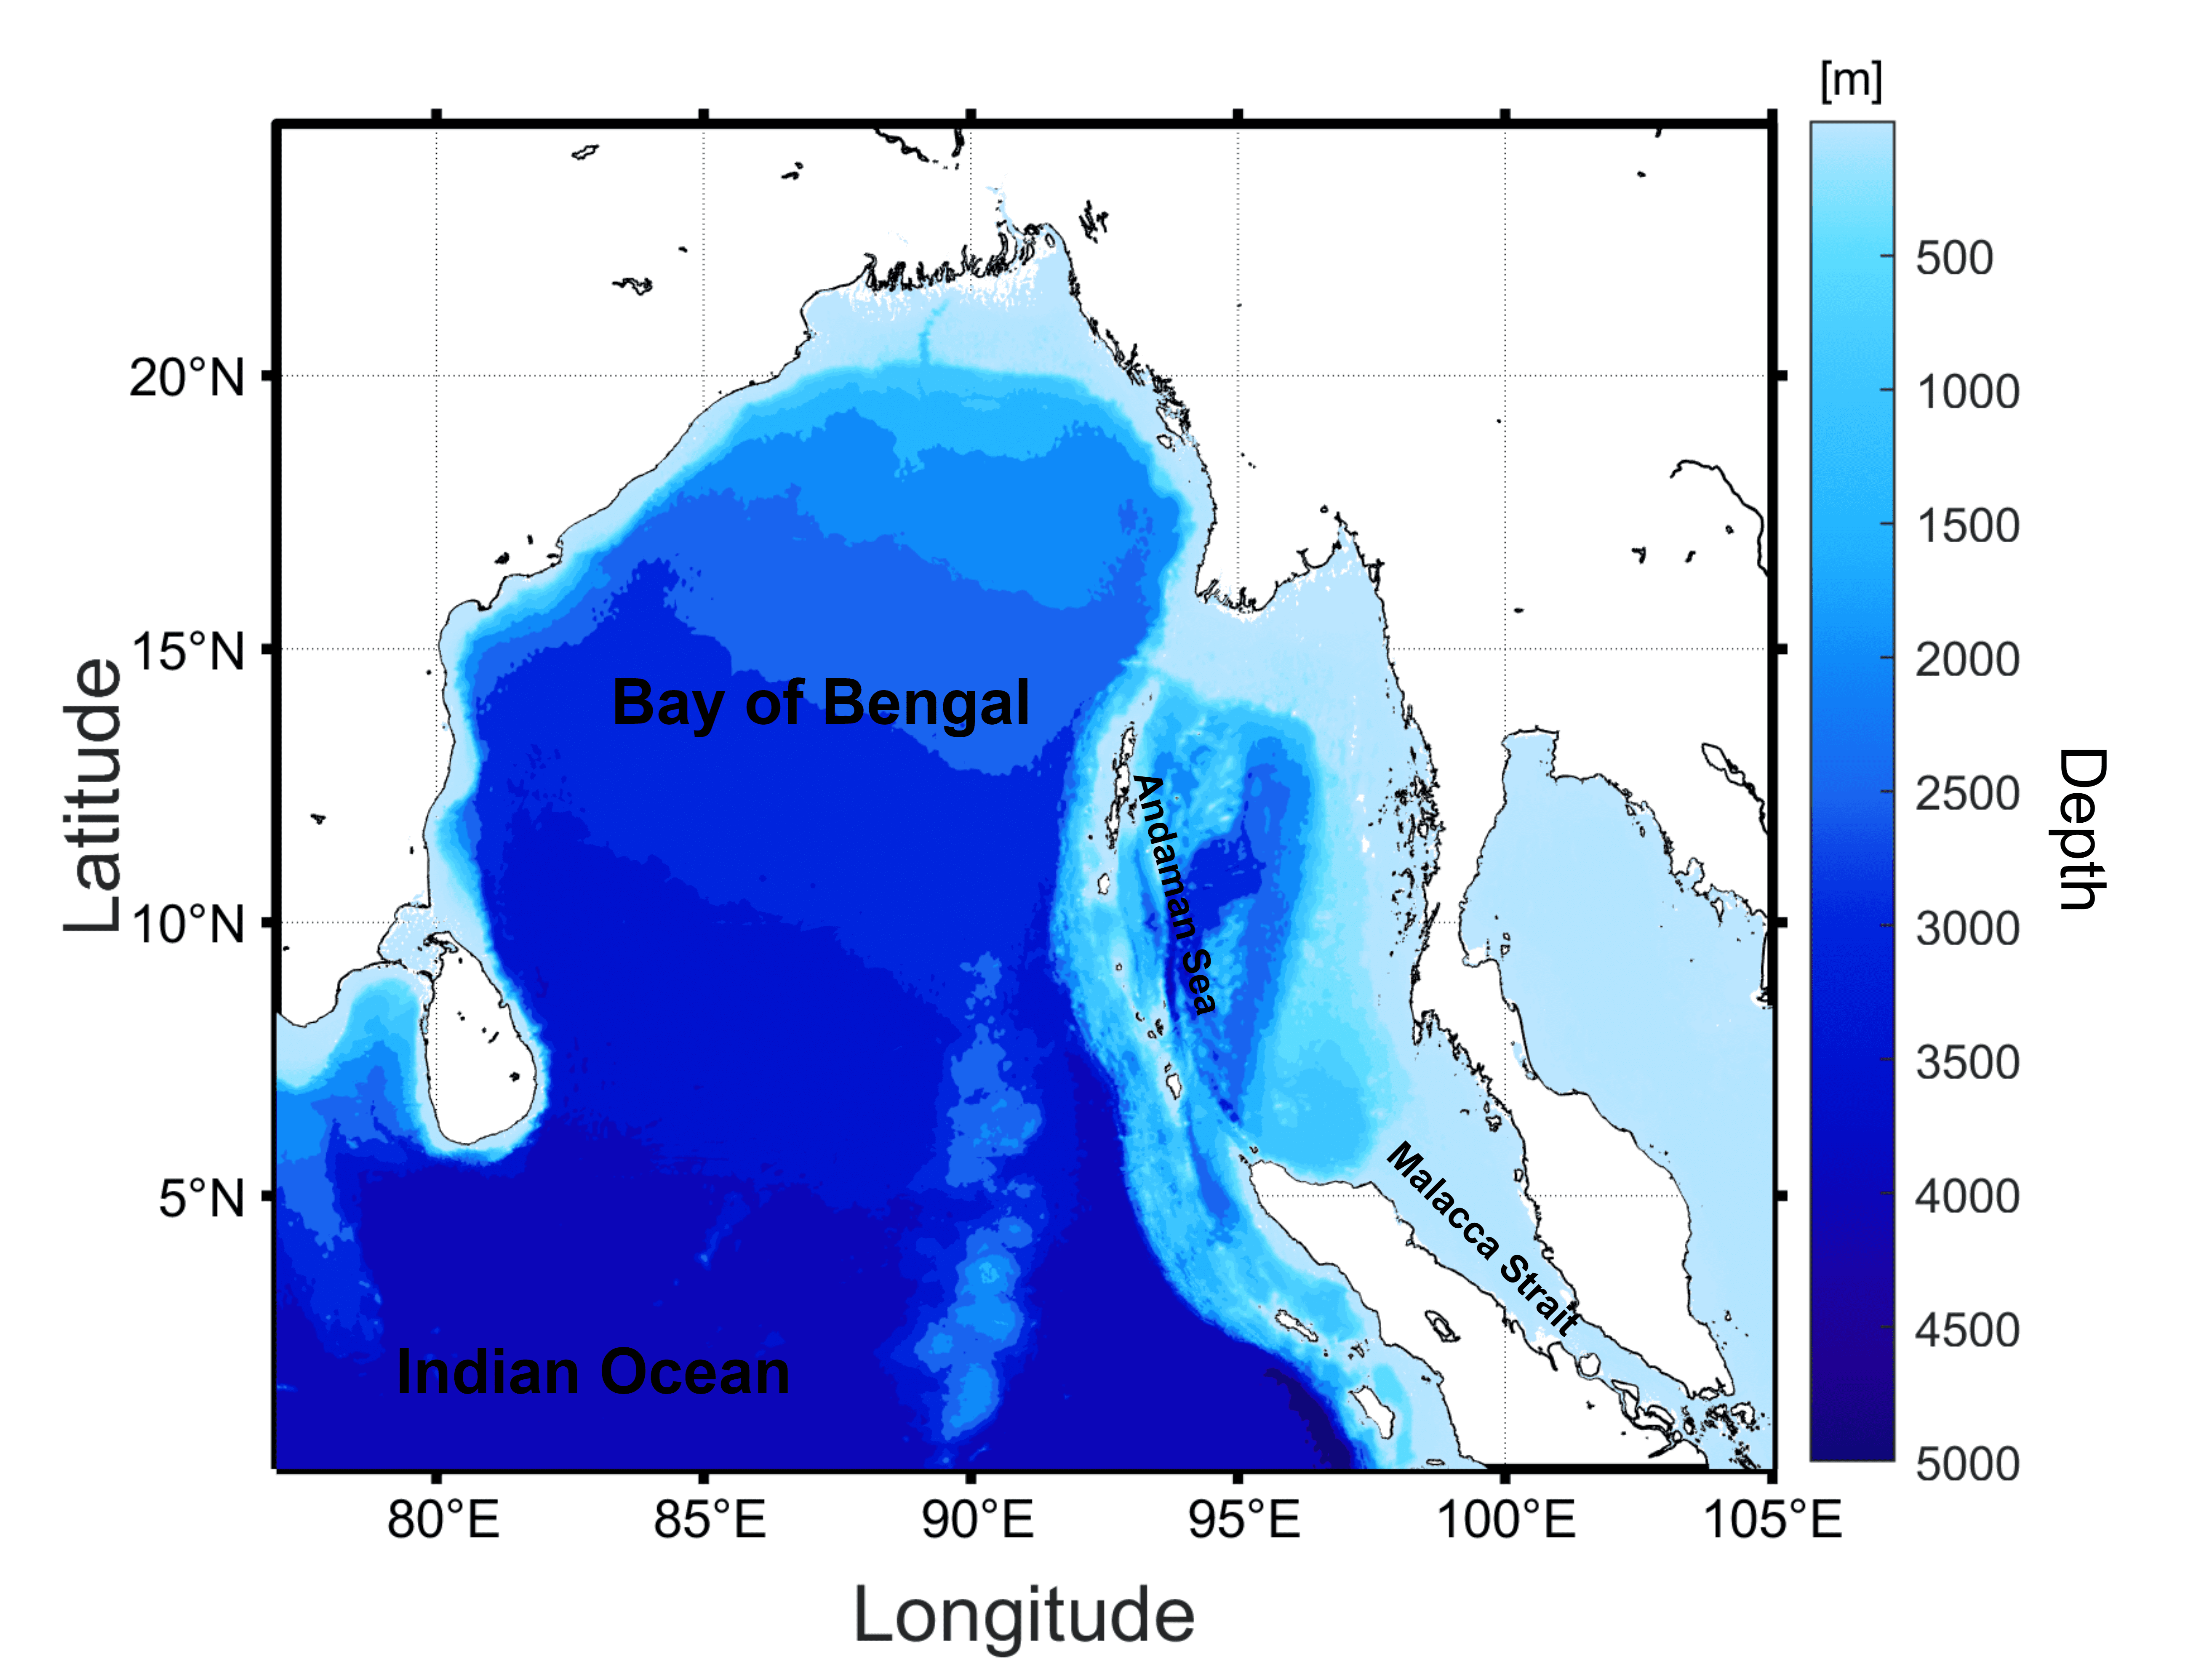
\includegraphics[width=12cm]{contents/Figures/Batimetri_edit_compress}
		\caption{Peta batimetri Samudera Hindia, diperoleh dari SRTM30+ \protect\cite{becker2009global}. Warna dalam peta menunjukkan kedalaman 0-5000 m sedangkan pulau digambarkan tanpa warna.}
		\label{fig:domain}
	\end{figure}
\end{spacing}
\vspace{-0.5pc}
\section[Analisis Data]{Analisis Data}
\begin{spacing}{1.5}
	\subsection[Model Musiman]{Model Musiman}

	Data jangka panjang dapat dianalisis dengan menggunakan analisis deret waktu, sebagai contoh analisis model musiman, yang bertujuan untuk menganalisis kemungkinan adanya pola musiman yang berulang dalam periode tertentu pada data tersebut. Monsun merupakan penyebab utama perubahan IOD, parameter oseanografi seperti arus laut, temperatur laut, salinitas, MLD, Chl-a, fluks air tawar, dan fluks panas bersih, serta parameter meteorologi seperti laju presipitasi dan angin. Penelitian ini akan menganalisis parameter-parameter tersebut dengan menggunakan model musiman yang didasarkan pada pola kejadian monsun. Model musiman ini digunakan untuk mengamati pola periodik dan memprediksi parameter-parameter berdasarkan keteraturan mereka. Dengan cara ini, akan diketahui apakah parameter yang diteliti mengikuti pola monsun yang terjadi, apakah terjadi pergeseran bulanan pada masing-masing parameter dalam model musiman yang dibangun, serta apakah parameter-parameter tersebut mengikuti pola monsun yang sama.

	Beberapa penelitian yang menggunakan model musiman adalah \shortciteauthor{Haridhi2016} \citeyear{Haridhi2016} yang meneliti tentang hubungan antara SST dan \textit{net deployment} (ND) - penyebaran jaring nelayan pukat cincin tradisional. \shortciteauthor{Ikhwan2022} \citeyear{Ikhwan2022} dalam penelitiannya mengkaji tentang MLD di Laut Andaman (AS) menggunakan data SSS dari model 3-D \textit{Copernicus Marine Environment Monitoring Service} (CMEMS).  
	
	Setiap fungsi periodik dapat diuraikan menjadi penjumlahan gelombang sinus dan kosinus. Persamaan terkait hal ini disebut juga sebagai deret Fourier atau model Harmonik. Secara matematis hal ini dapat dituliskan sebagai \cite{goela2016time,hyndman2018forecasting} 
	\begin{equation}\label{eq:fs}
		y = \alpha + \sum_{k=1}^{N} \left[ \beta_k \sin(\frac{2\pi kt}{m})+\gamma_k \cos(\frac{2\pi kt}{m})\right]  + \epsilon,
	\end{equation}
	dengan $\alpha, \beta_k, \gamma_k,k,\text{ dan }m$ adalah konstanta pergeseran vertikal, koefisien komponen sinus, koefisien komponen kosinus, ordo atau frekuensi gelombang sinus dan kosinus, dan periode fungsi. Bentuk sederhana dari Pers. \ref{eq:fs} dapat dituliskan sebagai
	persamaan siklus musiman \cite{crawley2012r}
	\begin{equation}\label{eq:sm_}
		y = \alpha + \beta \sin(2\pi t)+\gamma \cos(2\pi t) + \epsilon,
	\end{equation}
	dengan $\alpha, \beta$, dan $\gamma$  adalah konstanta pergesaran vertikal, amplitudo dari gelombang sinus, dan amplitudo dari gelombang kosinus. Dalam persamaan ini, $t$ adalah waktu dan $\epsilon$ adalah elemen residual yang mewakili komponen \textit{white-noise} tidak beraturan dalam proses pengambilan data. Parameter-parameter yang tidak diketahui, yaitu $\alpha, \beta, $ dan $\gamma$, diperkirakan menggunakan metode kuadrat terkecil (\textit{ordinary least squares}) \cite{goela2016time}.
	
	Gambar \ref{fig:sm} merupakan ilustrasi persamaan \ref{eq:sm_} untuk nilai $\alpha,\beta$ dan $\gamma$ yang berbeda. Nilai $\alpha$ yang berbeda mempengaruhi posisi kurva terhadap sumbu-y. Sedangkan nilai $\beta$ dan $\gamma$ yang berbeda mempengaruhi posisi kurva terhadap sumbu-x.
	\begin{figure}[H]
		\centering
		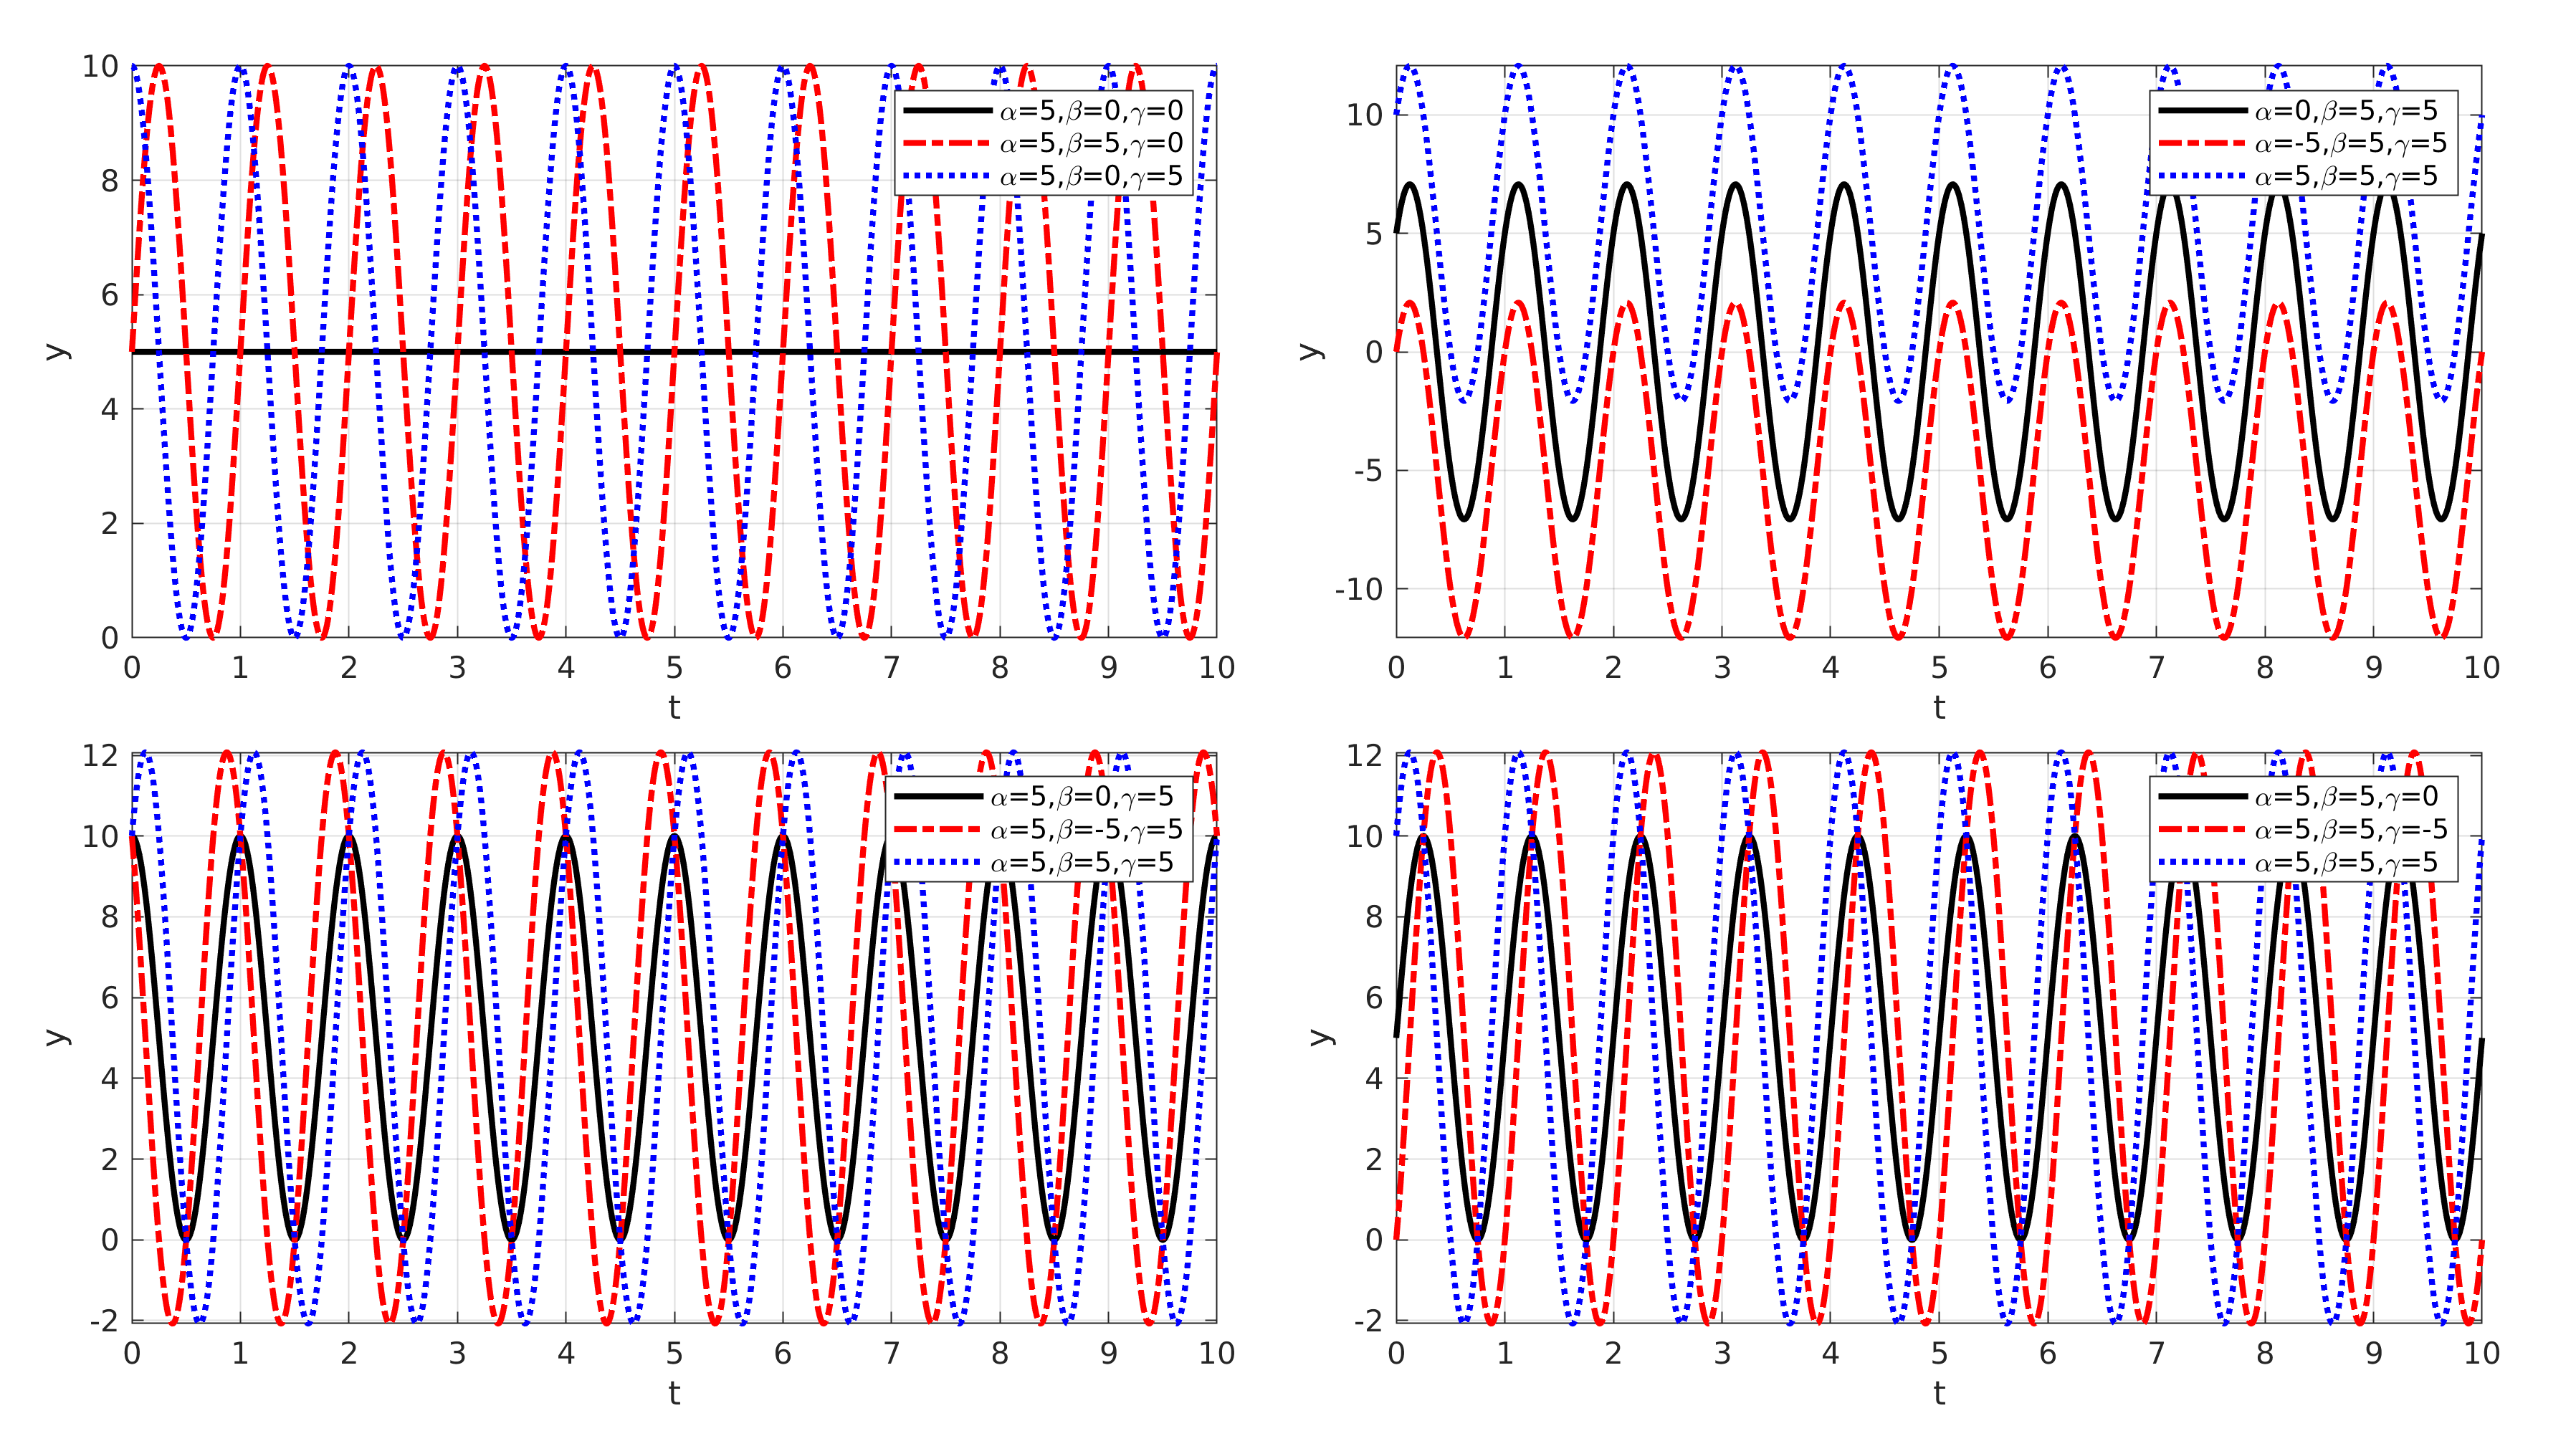
\includegraphics[width=15cm]{contents/Figures/sm_experiment}
		\caption{Ilustrasi persamaan model musiman.}
		\label{fig:sm}
	\end{figure}
	
%	Langkah-langkah yang digunakan untuk menggambarkan \textit{seasonal model} dapat dijelaskan sebagai berikut.
%	\begin{itemize}
%		\item \textbf{\textit{Start}}. \textit{Software} yang digunakan untuk menentukan nilai $\alpha, \beta$ dan $\gamma$ adalah \textit{software} \textit{R}.
%		\item \textbf{\textit{Initialization}}. Dalam proses inisialisasi ini, komponen musiman semua parameter dimodelkan untuk mendapatkan siklus tahunan.
%		\item \textbf{\textit{Input}}. Setelah proses inisialisasi \textit{input} parameter yang ingin diprediksi kemudian dimasukkan.
%		\item \textbf{\textit{Process}}. Selanjutnya dilakukan perhitungan dengan menggunakan fungsi model linear (\verb|lm()|) dalam \textit{R}.
%		\item \textbf{\textit{Output}}. Perintah Summary() digunakan untuk menampilkan hasil dalam proses sebelumnya. Dalam tahapan ini juga diperoleh penggambaran \textit{seasonal model}.
%	\end{itemize}

	\subsection[Analisis Korelasi]{Analisis Korelasi}
		Analisis korelasi berfungsi sebagai alat eksplorasi data dan pembuatan hipotesis dalam menentukan hubungan antara parameter yang diteliti. Dalam penelitian ini, analisis korelasi digunakan untuk mengukur kekuatan (nilai koefisien korelasi) dan arah (positif/negatif) hubungan antara indeks IOD dengan parameter lainnya, serta untuk menentukan signifikansi koefisien korelasi tersebut.
		
<<<<<<< HEAD
		Analisis korelasi mempelajari hubungan linier antara variabel/parameter yang diteliti. Jika terdapat hubungan antara dua karakteristik, langkah selanjutnya adalah mengevaluasi apakah variabel pertama dapat digunakan untuk memprediksi variabel kedua melalui analisis regresi. Kekuatan dari korelasi ditentukan berdasarkan koefisien korelasi ($R$), yang bervariasi antara -1 dan +1. Berdasarkan \citeA{schober2018correlation}, jika $R\in[0.00,0.10]$ maka korelasi diabaikan. Jika $R\in[0.10,0.39]$ maka korelasi lemah. Jika $R\in[0.40,0.69]$ maka korelasi kuat. Jika $R\in[0.90,1.00]$ maka korelasi sangat kuat. Sementara itu, arah dari korelasi dapat berupa korelasi positif atau korelasi negatif. Korelasi positif terjadi jika nilai variabel pertama berbanding lurus dengan variabel kedua. Sedangkan korelasi negatif terjadi jika nilai variabel pertama berbanding terbalik dengan variabel kedua. Persamaan koefisien korelasi dapat dituliskan sebagai berikut  \cite{hidayat2023relationship,Haditiar2020,zhao2022spearman}.
		\begin{itemize}
			\item Korelasi Pearson
			\begin{equation}
				\begin{aligned}
					R &= \frac{\sum (x_i - \bar{x})(y_i - \bar{y})}{\sqrt{\sum (x_i-\bar{x})^2\sum (y_i-\bar{y})^2}},
				\end{aligned}
			\end{equation}
			dengan $x_i, y_i$ adalah variable yang digunakan untuk menghitung koefisien korelasi dengan $i$ adalah indeks data. Sedangkan $\bar{x}$ dan $\bar{y}$ adalah rata-rata. Analisis korelasi Pearson merupakan korelasi linear antara variabel yang berukuran metrik.
			\item Korelasi Spearman
			\begin{equation}
				\begin{aligned}
					%				y &= b+ax\\
					R_s &= 1-\frac{6\cdot\sum d_i^2}{n\cdot(n^2-1)},
				\end{aligned}
			\end{equation}
			dengan $n$ adalah jumlah kasus dan $d_i$ adalah perbedaan peringkat antara dua variabel. Korelasi Spearman adalah pendamping non-parametrik dari korelasi Pearson.
		\end{itemize}
	
		Untuk menggunakan korelasi Pearson, variabel harus terdistribusi secara normal dan harus terdapat hubungan linear antara variabel-variabel tersebut. Distribusi normal dapat diuji baik secara analitis maupun grafis dengan menggunakan plot QQ (\textit{Quantile-Quantile plot}) sedangkan korelasi linear dapat diperiksa dengan menggunakan scatter plot. Jika kondisi-kondisi ini tidak terpenuhi, maka digunakan korelasi Spearman.
=======
		Penelitian ini menganalisis hubungan antara IOD, parameter oseanografi (arus laut, temperatur laut, salinitas, MLD, Chl-a, fluks air tawar, fluks panas bersih) dan meteorologi (laju presipitasi dan tekanan angin). Persamaan korelasi dan koefisien korelasi yang digunakan dapat dituliskan sebagai \cite{Haditiar2020}
		\begin{equation}
			\begin{aligned}
				y &= a+rx\\
				r &= \frac{\sum (x_i - \bar{x})(y_i - \bar{y})}{\sqrt{\sum (x_i-\bar{x})^2\sum (y_i-\bar{y})^2}},
			\end{aligned}
		\end{equation}
		dengan $\alpha$ adalah konstanta titik potong sumbu-$y$, $r$ adalah kemiringan dari garis regresi (koefisien regresi), $x_i, y_i$ adalah variable yang digunakan untuk menghitung koefisien korelasi dengan $i$ adalah indeks data. Sedangkan $\bar{x}$ dan $\bar{y}$ adalah rata-rata. 
>>>>>>> 78c771c8721f1c7bc670f04aed28e27a85f35326
		
		Signifikansi dari koefisien korelasi diuji dengan uji t dengan cara menguji apakah koefisien korelasi secara signifikan berbeda dari nol (uji bebas linier). Dalam hal ini, hipotesis nol menyatakan tidak ada korelasi antara variabel yang dipertimbangkan, sementara hipotesis alternatif mengasumsikan adanya korelasi. Dengan tingkat signifikansi $(\alpha)$ pada 1\% atau 5\%, jika nilai p < 5\%, hipotesis nol ditolak dan hipotesis alternatif diterima yang berarti bahwa terdapat hubungan antara variabel dalam populasi. Persamaan untuk t-statistik dapat dituliskan sebagai
		\begin{equation}
			\begin{aligned}
				t=\frac{R\sqrt{n-2}}{1-R^2}.
			\end{aligned}
		\end{equation}
		dengan $n$ ukuran sampel dan $R$ korelasi yang ditentukan dalam sampel.
		\subsection[Analisis Regresi]{Analisis Regresi}
		Analisis regresi memungkinkan pemodelan hubungan antara variabel dependen dan satu atau lebih variabel independen. Dengan analisis regresi, dapat diketahui ukuran pengaruh satu atau lebih variabel terhadap variabel lain serta dapat memprediksi sebuah variabel berdasarkan satu atau lebih variabel lainnya. Hal ini karena analisis regresi memberikan informasi tentang bagaimana nilai variabel dependen berubah jika salah satu variabel independen diubah. Analisis regresi dibedakan sebagai berikut  \cite{ANGELINI2019722}.
		\begin{itemize}
			\item Regresi Linear Sederhana
			\begin{equation}
				\begin{aligned}
					y &= a \cdot x+b\\
				\end{aligned}
			\end{equation}
			dengan $y$ dan $x$ adalah variabel dependen dan independen, $b$ adalah konstanta titik potong sumbu-$y$, dan $a$ adalah koefisien regresi yang mengukur pengaruh variabel independen $(x)$ terhadap variabel dependen $(y)$.
			\item Regresi Linier Berganda
			\begin{equation}
				\begin{aligned}
					y &= a_1 \cdot x_1+a_2 \cdot x_2+\dots+a_k \cdot x_k+b,
				\end{aligned}
			\end{equation}
			dengan $y$ dan $x_1,x_2,\dots,x_k$ adalah variabel dependen dan independen, $b$ adalah konstanta titik potong sumbu-$y$, dan $a_1,a_2,\dots,a_k$ adalah koefisien regresi yang mengukur pengaruh variabel independen $(x_1,x_2,\dots,x_k)$ terhadap variabel dependen $(y)$.
		\end{itemize}

\end{spacing}
\vspace{-0.5pc}
\section[Prosedur Penelitian]{Prosedur Penelitian}
\begin{spacing}{1.5}
	Prosedur penelitian mengikuti diagram alir pada Gambar \ref{fig:flowchart} dan dapat dijelaskan sebagai berikut. 
	\begin{itemize}
		\item \textbf{\textit{Start}}. \textit{Software} yang digunakan dalam penelitian ini adalah Matlab dan \textit{R}.
		\item \textbf{\textit{Input}}. Data penelitian diunduh terlebih dahulu. Adapun data yang digunakan adalah data DMI, arus laut, temperatur laut, salinitas, MLD, Chl-a, fluks air tawar, fluks panas bersih, laju presipitasi, dan tekanan angin.
		\item \textbf{\textit{Process}}. Data kemudian diolah dengan cara melakukan pemetaan dan penggambaran data. Pada tahap ini akan dilakukan beberapa hal berikut.
		\begin{itemize}
			\item Prapemrosesan data, yaitu mempersiapkan data sebelum dipetakan dan digambar.
			\item Pemetaan data, yaitu proses memetakan atau menetapkan data dari satu format ke format lain atau dari satu lokasi ke lokasi lain dengan tujuan untuk memudahkan pengolahan data, sehingga dapat digunakan untuk tujuan analisis atau pelaporan.
			\item Pembersihan data, yaitu proses mengidentifikasi, mengubah, atau menghapus data yang tidak akurat, tidak lengkap, atau tidak relevan dalam kumpulan data. 
			\item Penggambaran data, yaitu proses menyajikan data dalam bentuk visual, seperti grafik, diagram, atau peta dengan tujuan untuk memudahkan pemahaman dan analisis terhadap data yang kompleks dan memudahkan untuk melihat pola dan tren dari data yang disajikan.
		\end{itemize}
		
		\item \textbf{\textit{Output}}. Penggambaran data pada tahap sebelumnya menghasilkan peta IOD, oseanografi, dan meteorologi secara jangka panjang. 
		\item \textbf{\textit{Process}}. Dalam tahap ini akan dilakukan beberapa analisis data, diantaranya model musiman (\textit{seasonal model}) untuk mengidentifikasi pola musiman dan memprediksi parameter berdasarkan keteraturannya dan analisis korelasi untuk mengukur kekuatan dan arah hubungan antara IOD dengan parameter oseanografi dan meteorologi, serta untuk menentukan signifikansi koefisien korelasi tersebut.
		
%		Tahapan yang dilakukan dalam analisis \textit{seasonal model} dapat dijelaskan sebagai berikut.
%		\begin{itemize}
%			\item Input: data DMI, arus laut, temperatur laut, salinitas, MLD, Chl-a, fluks air tawar, fluks panas bersih, laju presipitasi, dan tekanan angin.
%			\item Pemodelan komponen musiman: Pada tahap ini, nilai $\alpha, \beta$, dan $\gamma$ pada Pers. \ref{eq:sm_} akan ditentukan dengan menggunakan fungsi model linear (lm()) dalam R. Nilai ini kemudian digunakan untuk memodelkan komponen musiman.
%			\item \textit{Plotting Model}: Setelah komponen musiman dimodelkan, langkah selanjutnya adalah melakukan \textit{plotting model} untuk memvisualisasikan hasil analisis.
%		\end{itemize}
		
%		Tahapan yang dilakukan dalam analisis korelasi dapat dijelaskan sebagai berikut.
%		\begin{itemize}
%			\item Tentukan hipotesis nol dan hipotesis alternatif.
%			\item Tentukan tingkat signifikansi alpha (alpha 1\% atau 5\%).
%			\item Hitung koefisien korelasi antara dua variabel.
%			\item Hitung nilai p (nilai probabilitas) dari koefisien korelasi untuk menentukan signifikansi statistik.
%			\item Bandingkan nilai p dengan tingkat signifikansi $\alpha$. Jika p < $\alpha$, maka korelasi signifikan secara statistik dan hipotesis nol dapat ditolak. Sedangkan jika p > $\alpha$, maka tidak ada bukti yang cukup untuk menolak hipotesis nol dan korelasi dianggap tidak signifikan.
%			\item Plot hasil uji korelasi.
%		\end{itemize}
		\item \textbf{\textit{Output}}. Dari proses analisis data diperoleh peta seasonal model, peta korelasi, dan tabulasi hasil.
		\item \textbf{\textit{Process}}. Hasil output dari peta-peta IOD, oseanografi, meteorologi, model musiman, korelasi, dan tabulasi kemudian diinterpretasikan dan dituliskan dalam laporan.
		\item \textbf{\textit{End}}. Penelitian selesai.
	\end{itemize}
	\begin{figure}[H]
		\centering
		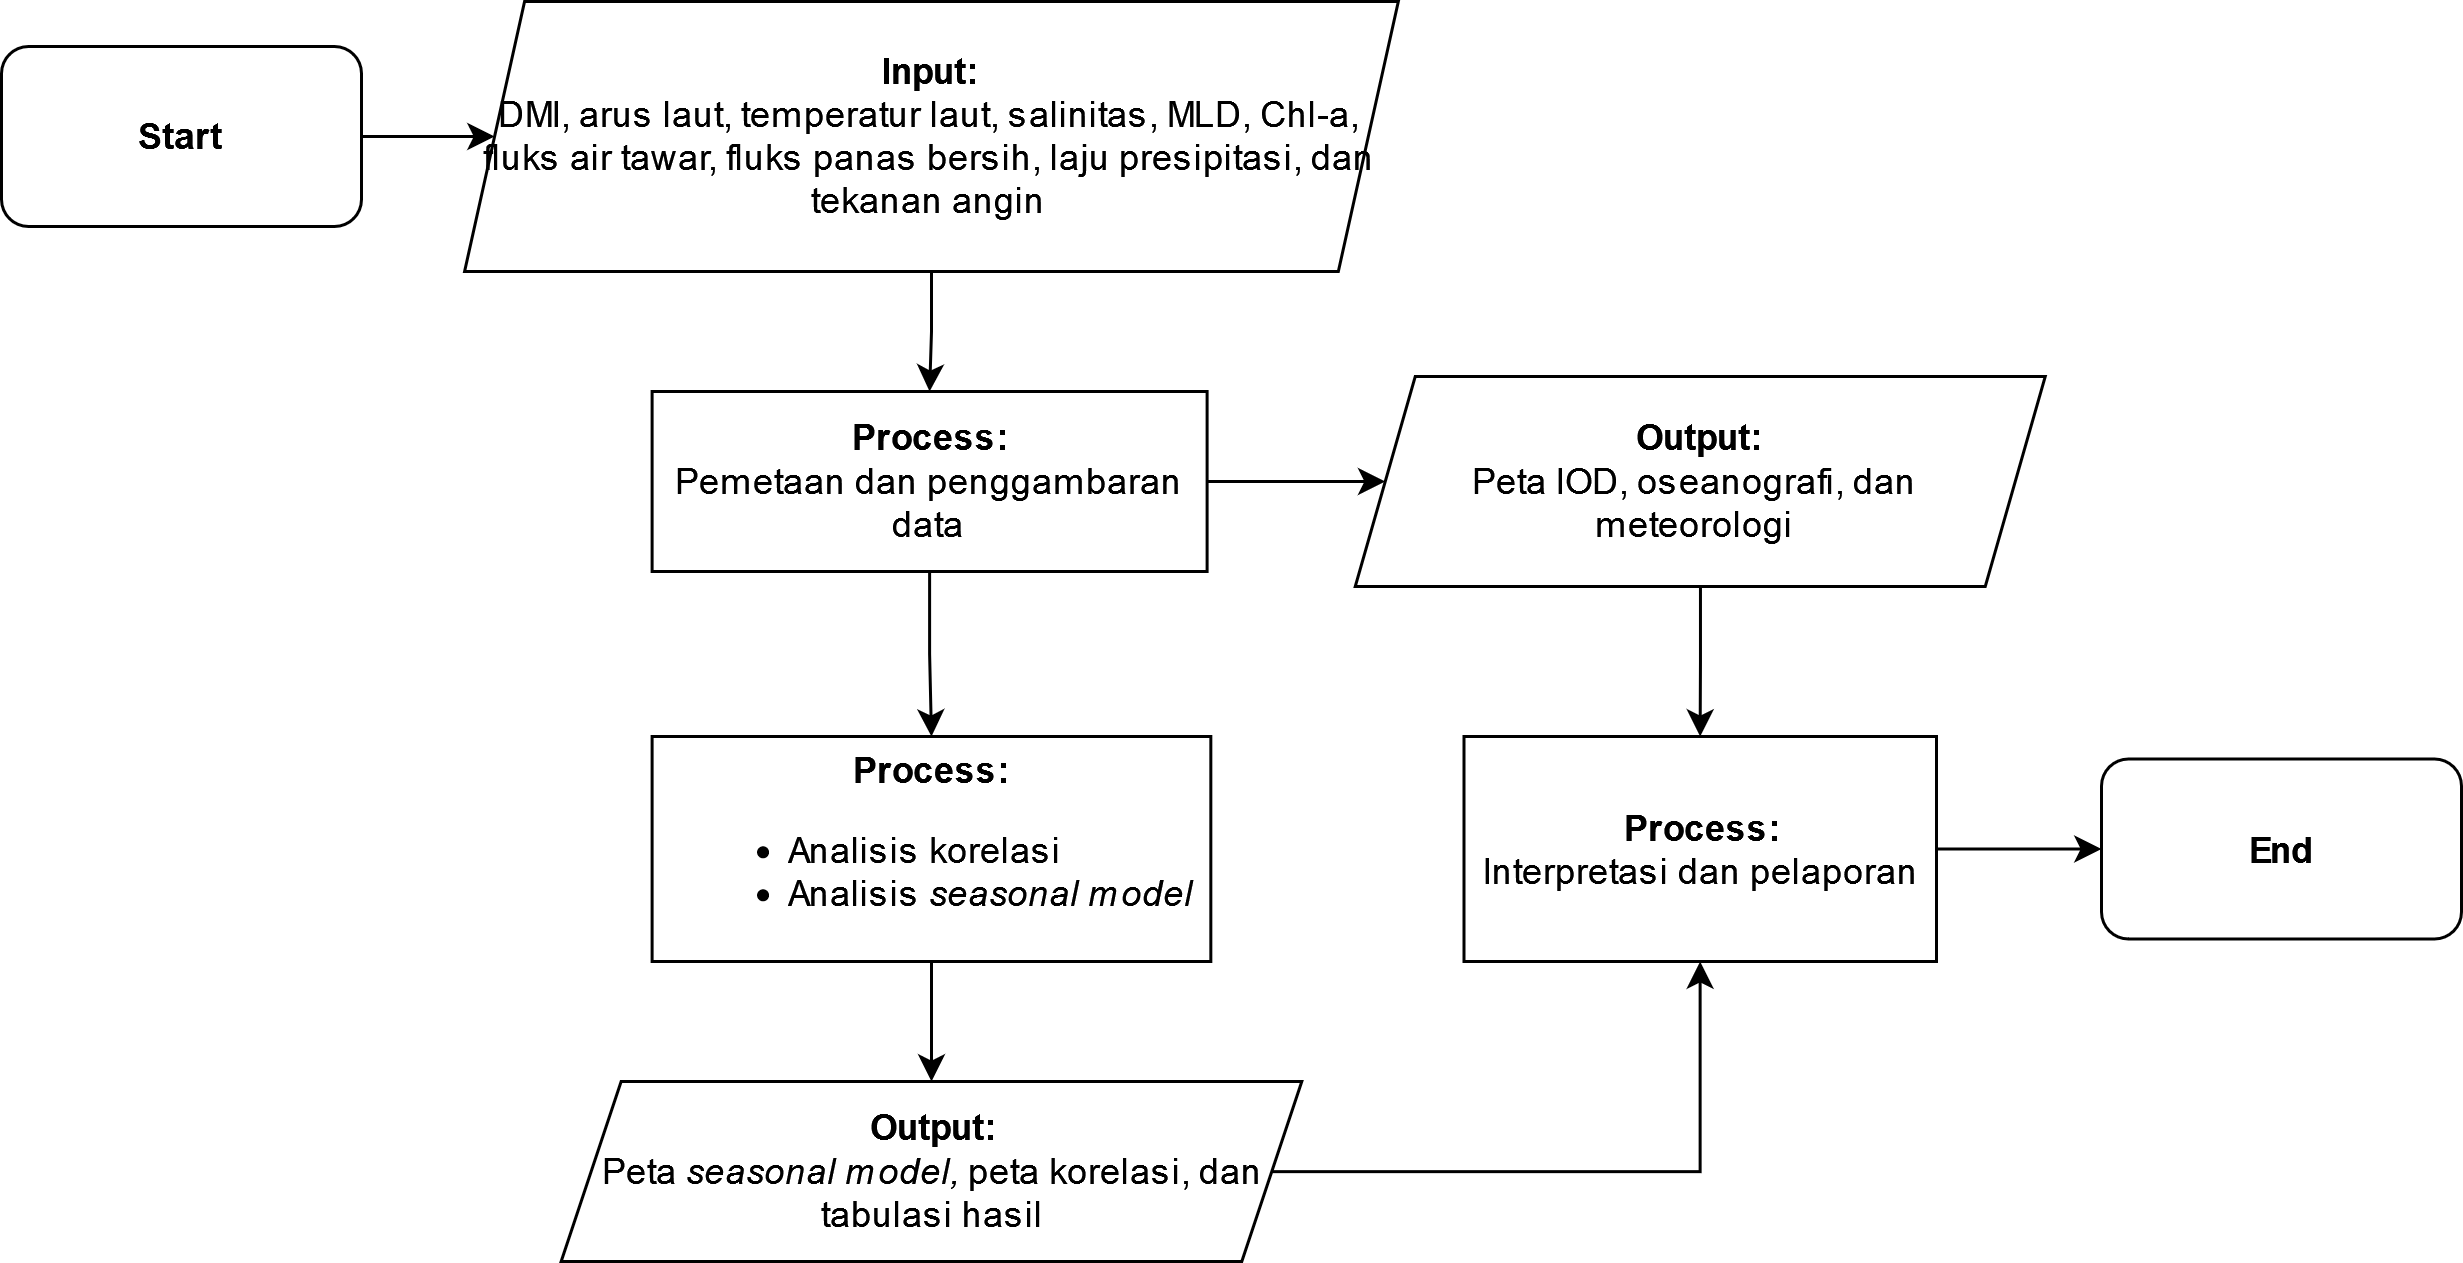
\includegraphics[width=14cm]{contents/Figures/Flowchart_Diagram.png}
		\caption{Diagram alir penelitian}
		\label{fig:flowchart}
	\end{figure}
\end{spacing}

%=====================================================================
% Halaman Output
\pagebreak
\chapter{BIAYA DAN JADWAL PENELITIAN}
\vspace{1.5pc}
\section[Biaya Penelitian]{Biaya Penelitian}
\begin{spacing}{1.5}
	Ringkasan anggaran biaya penelitian selama 3 tahun dapat dilihat pada Tabel \ref{tab:ang-pen}.
	% Please add the following required packages to your document preamble:
	% \usepackage[normalem]{ulem}
	% \useunder{\uline}{\ul}{}
	\begin{table}[htp]
		\caption{Ringkasan anggaran biaya penelitian}
		\centering
		\label{tab:ang-pen}
		\begin{tabular}{|ll|l|}
			\hline
			\multicolumn{1}{|l|}{No} & Jenis Pengeluaran                                                                                                                                                                                        & \begin{tabular}[c]{@{}l@{}}Biaya yang \\ diusulkan (Rp)\end{tabular} \\ \hline
			\multicolumn{1}{|l|}{1}  & \begin{tabular}[c]{@{}l@{}}Honorarium untuk pelaksana, petugas laboratorium, \\ pengumpul data, pengolah data, dan penganalisis data.\end{tabular}                                                       & 19.500.000                                                           \\ \hline
			\multicolumn{1}{|l|}{2}  & \begin{tabular}[c]{@{}l@{}}Pembelian bahan habis pakai untuk ATK, fotocopy, \\ surat menyurat, penyusunan laporan, cetak, penjilidan,\\ publikasi, pulsa, internet, dan bahan laboratorium.\end{tabular} & 71.400.000                                                           \\ \hline
			\multicolumn{1}{|l|}{3}  & \begin{tabular}[c]{@{}l@{}}Perjalanan untuk biaya survei/sampling data, seminar/\\ workshop DN-LN, biaya akomodasi, konsumsi, \\ perdiem/lumpsum, transport.\end{tabular}                                & 59.100.000                                                           \\ \hline
			\multicolumn{1}{|l|}{4}  & \begin{tabular}[c]{@{}l@{}}Sewa untuk peralatan/mesin/ruang laboratorium, \\ kendaraan, dan peralatan penunjang penelitian lainnya.\end{tabular}                                                         & 0                                                                    \\ \hline
			\multicolumn{2}{|c|}{Total}                                                                                                                                                                                                         & 150.000.000                                                           \\ \hline
		\end{tabular}
	\end{table}
\end{spacing}
\vspace{-0.5pc}
\pagebreak 
\section[Jadwal Penelitian]{Jadwal Penelitian}
\begin{spacing}{1.5}
	Jadwal penelitian disusun berdasarkan lama studi yang telah ditempuh dan akan ditempuh. Penelitian diusulkan dalam tiga tahun, dengan rincian kegiatan sebagaimana tertera dalam Tabel \ref{tab:jad-pen}.
	% Please add the following required packages to your document preamble:
% \usepackage{multirow}
% \usepackage[table,xcdraw]{xcolor}
% If you use beamer only pass "xcolor=table" option, i.e. \documentclass[xcolor=table]{beamer}
\begin{table}[htp]
	\caption{Ringkasan jadwal pelaksanaan penelitian}
	\centering
	\label{tab:jad-pen}
	\begin{tabular}{|l|l|llllllllllll|}
		\hline
		\multicolumn{1}{|c|}{}                     &                                                                                      & \multicolumn{12}{c|}{Tahun I}                                                                                                                                                                                                                                                                                                                                                                                                                                                                                                                                            \\ \cline{3-14} 
		\multicolumn{1}{|c|}{\multirow{-2}{*}{No}} & \multirow{-2}{*}{Kegiatan}                                                           & \multicolumn{1}{c|}{1}                        & \multicolumn{1}{c|}{2}                        & \multicolumn{1}{c|}{3}                        & \multicolumn{1}{c|}{4}                        & \multicolumn{1}{c|}{5}                        & \multicolumn{1}{c|}{6}                        & \multicolumn{1}{c|}{7}                        & \multicolumn{1}{c|}{8}                        & \multicolumn{1}{c|}{9}                        & \multicolumn{1}{c|}{10}                       & \multicolumn{1}{c|}{11}                       & \multicolumn{1}{c|}{12}  \\ \hline
		1                                          & Studi literatur                                                                      & \multicolumn{1}{l|}{\cellcolor[HTML]{343434}} & \multicolumn{1}{l|}{\cellcolor[HTML]{343434}} & \multicolumn{1}{l|}{\cellcolor[HTML]{343434}} & \multicolumn{1}{l|}{\cellcolor[HTML]{343434}} & \multicolumn{1}{l|}{}                         & \multicolumn{1}{l|}{}                         & \multicolumn{1}{l|}{}                         & \multicolumn{1}{l|}{}                         & \multicolumn{1}{l|}{}                         & \multicolumn{1}{l|}{}                         & \multicolumn{1}{l|}{}                         &                          \\ \hline
		2                                          & Penyusunan proposal                                                                  & \multicolumn{1}{l|}{}                         & \multicolumn{1}{l|}{}                         & \multicolumn{1}{l|}{}                         & \multicolumn{1}{l|}{}                         & \multicolumn{1}{l|}{\cellcolor[HTML]{343434}} & \multicolumn{1}{l|}{\cellcolor[HTML]{343434}} & \multicolumn{1}{l|}{\cellcolor[HTML]{343434}} & \multicolumn{1}{l|}{\cellcolor[HTML]{343434}} & \multicolumn{1}{l|}{}                         & \multicolumn{1}{l|}{}                         & \multicolumn{1}{l|}{}                         &                          \\ \hline
		3                                          & \begin{tabular}[c]{@{}l@{}}Persiapan data model \\ dan data observasi\end{tabular}   & \multicolumn{1}{l|}{}                         & \multicolumn{1}{l|}{}                         & \multicolumn{1}{l|}{}                         & \multicolumn{1}{l|}{}                         & \multicolumn{1}{l|}{}                         & \multicolumn{1}{l|}{}                         & \multicolumn{1}{l|}{}                         & \multicolumn{1}{l|}{}                         & \multicolumn{1}{l|}{\cellcolor[HTML]{343434}} & \multicolumn{1}{l|}{\cellcolor[HTML]{343434}} & \multicolumn{1}{l|}{\cellcolor[HTML]{343434}} &                          \\ \hline
		4                                          & Pemrosesan data                                                                      & \multicolumn{1}{l|}{}                         & \multicolumn{1}{l|}{}                         & \multicolumn{1}{l|}{}                         & \multicolumn{1}{l|}{}                         & \multicolumn{1}{l|}{}                         & \multicolumn{1}{l|}{}                         & \multicolumn{1}{l|}{}                         & \multicolumn{1}{l|}{}                         & \multicolumn{1}{l|}{}                         & \multicolumn{1}{l|}{}                         & \multicolumn{1}{l|}{}                         & \cellcolor[HTML]{343434} \\ \hline
		\multicolumn{1}{|c|}{}                     &                                                                                      & \multicolumn{12}{c|}{Tahun II}                                                                                                                                                                                                                                                                                                                                                                                                                                                                                                                                           \\ \cline{3-14} 
		\multicolumn{1}{|c|}{\multirow{-2}{*}{No}} & \multirow{-2}{*}{Kegiatan}                                                           & \multicolumn{1}{c|}{1}                        & \multicolumn{1}{c|}{`2}                       & \multicolumn{1}{c|}{3}                        & \multicolumn{1}{c|}{4}                        & \multicolumn{1}{c|}{5}                        & \multicolumn{1}{c|}{6}                        & \multicolumn{1}{c|}{7}                        & \multicolumn{1}{c|}{8}                        & \multicolumn{1}{c|}{9}                        & \multicolumn{1}{c|}{10}                       & \multicolumn{1}{c|}{11}                       & \multicolumn{1}{c|}{12}  \\ \hline
		5                                          & Pemrosesan data lanjutan                                                             & \multicolumn{1}{l|}{\cellcolor[HTML]{343434}} & \multicolumn{1}{l|}{\cellcolor[HTML]{343434}} & \multicolumn{1}{l|}{}                         & \multicolumn{1}{l|}{}                         & \multicolumn{1}{l|}{}                         & \multicolumn{1}{l|}{}                         & \multicolumn{1}{l|}{}                         & \multicolumn{1}{l|}{}                         & \multicolumn{1}{l|}{}                         & \multicolumn{1}{l|}{}                         & \multicolumn{1}{l|}{}                         &                          \\ \hline
		6                                          & Hasil dan analisis                                                                   & \multicolumn{1}{l|}{}                         & \multicolumn{1}{l|}{}                         & \multicolumn{1}{l|}{\cellcolor[HTML]{343434}} & \multicolumn{1}{l|}{\cellcolor[HTML]{343434}} & \multicolumn{1}{l|}{}                         & \multicolumn{1}{l|}{}                         & \multicolumn{1}{l|}{}                         & \multicolumn{1}{l|}{}                         & \multicolumn{1}{l|}{}                         & \multicolumn{1}{l|}{}                         & \multicolumn{1}{l|}{}                         &                          \\ \hline
		7                                          & Publikasi 1                                                                          & \multicolumn{1}{l|}{}                         & \multicolumn{1}{l|}{}                         & \multicolumn{1}{l|}{}                         & \multicolumn{1}{l|}{}                         & \multicolumn{1}{l|}{\cellcolor[HTML]{343434}} & \multicolumn{1}{l|}{\cellcolor[HTML]{343434}} & \multicolumn{1}{l|}{\cellcolor[HTML]{343434}} & \multicolumn{1}{l|}{}                         & \multicolumn{1}{l|}{}                         & \multicolumn{1}{l|}{}                         & \multicolumn{1}{l|}{}                         &                          \\ \hline
		8                                          & Studi literatur lanjutan                                                             & \multicolumn{1}{l|}{}                         & \multicolumn{1}{l|}{}                         & \multicolumn{1}{l|}{}                         & \multicolumn{1}{l|}{}                         & \multicolumn{1}{l|}{}                         & \multicolumn{1}{l|}{}                         & \multicolumn{1}{l|}{}                         & \multicolumn{1}{l|}{\cellcolor[HTML]{343434}} & \multicolumn{1}{l|}{\cellcolor[HTML]{343434}} & \multicolumn{1}{l|}{\cellcolor[HTML]{343434}} & \multicolumn{1}{l|}{}                         &                          \\ \hline
		9                                          & Hasil dan analisis                                                                   & \multicolumn{1}{l|}{}                         & \multicolumn{1}{l|}{}                         & \multicolumn{1}{l|}{}                         & \multicolumn{1}{l|}{}                         & \multicolumn{1}{l|}{}                         & \multicolumn{1}{l|}{}                         & \multicolumn{1}{l|}{}                         & \multicolumn{1}{l|}{}                         & \multicolumn{1}{l|}{}                         & \multicolumn{1}{l|}{\cellcolor[HTML]{343434}} & \multicolumn{1}{l|}{\cellcolor[HTML]{343434}} & \cellcolor[HTML]{343434} \\ \hline
		\multicolumn{1}{|c|}{}                     &                                                                                      & \multicolumn{12}{c|}{Tahun III}                                                                                                                                                                                                                                                                                                                                                                                                                                                                                                                                          \\ \cline{3-14} 
		\multicolumn{1}{|c|}{\multirow{-2}{*}{No}} & \multirow{-2}{*}{Kegiatan}                                                           & \multicolumn{1}{c|}{1}                        & \multicolumn{1}{c|}{2}                        & \multicolumn{1}{c|}{3}                        & \multicolumn{1}{c|}{4}                        & \multicolumn{1}{c|}{5}                        & \multicolumn{1}{c|}{6}                        & \multicolumn{1}{c|}{7}                        & \multicolumn{1}{c|}{8}                        & \multicolumn{1}{c|}{9}                        & \multicolumn{1}{c|}{10}                       & \multicolumn{1}{c|}{11}                       & \multicolumn{1}{c|}{12}  \\ \hline
		10                                         & Publikasi 2                                                                          & \multicolumn{1}{l|}{\cellcolor[HTML]{343434}} & \multicolumn{1}{l|}{\cellcolor[HTML]{343434}} & \multicolumn{1}{l|}{\cellcolor[HTML]{343434}} & \multicolumn{1}{l|}{\cellcolor[HTML]{343434}} & \multicolumn{1}{l|}{}                         & \multicolumn{1}{l|}{}                         & \multicolumn{1}{l|}{}                         & \multicolumn{1}{l|}{}                         & \multicolumn{1}{l|}{}                         & \multicolumn{1}{l|}{}                         & \multicolumn{1}{l|}{}                         &                          \\ \hline
		11                                         & \begin{tabular}[c]{@{}l@{}}Studi literatur untuk \\ penulisan disertasi\end{tabular} & \multicolumn{1}{l|}{}                         & \multicolumn{1}{l|}{}                         & \multicolumn{1}{l|}{}                         & \multicolumn{1}{l|}{}                         & \multicolumn{1}{l|}{\cellcolor[HTML]{343434}} & \multicolumn{1}{l|}{\cellcolor[HTML]{343434}} & \multicolumn{1}{l|}{\cellcolor[HTML]{343434}} & \multicolumn{1}{l|}{}                         & \multicolumn{1}{l|}{}                         & \multicolumn{1}{l|}{}                         & \multicolumn{1}{l|}{}                         &                          \\ \hline
		12                                         & Penyusunan disertasi                                                                 & \multicolumn{1}{l|}{}                         & \multicolumn{1}{l|}{}                         & \multicolumn{1}{l|}{}                         & \multicolumn{1}{l|}{}                         & \multicolumn{1}{l|}{}                         & \multicolumn{1}{l|}{}                         & \multicolumn{1}{l|}{}                         & \multicolumn{1}{l|}{\cellcolor[HTML]{343434}} & \multicolumn{1}{l|}{\cellcolor[HTML]{343434}} & \multicolumn{1}{l|}{}                         & \multicolumn{1}{l|}{}                         &                          \\ \hline
	\end{tabular}
\end{table}
\end{spacing}
%=====================================================================
% BAB IV
%\chapter{HASIL DAN PEMBAHASAN}
%\vspace{1.5pc}
\vspace{1.5pc}
\section[Hasil 1]{HASIL 1}
\begin{spacing}{1.5}
	
	\lipsum[1-4]
	
\end{spacing}
%=====================================================================
% BAB V
%\chapter{PENUTUP}
%\vspace{1.5pc}
\vspace{1.5pc}
\begin{spacing}{1.5}
\section[Kesimpulan]{KESIMPULAN}

\lipsum[2-4]

\section[Saran]{SARAN}

\lipsum[2-4]\cite{Adams2011}

\end{spacing}
%=====================================================================
% Halaman Daftar Pustaka
\pagebreak
%\addcontentsline{toc}{chapter}{\textbf{DAFTAR PUSTAKA}}
\renewcommand\bibname{DAFTAR PUSTAKA}	
\bibliographystyle{packages/apacite}
\bibliography{contents/ReferenceMendeley.bib}
%\{DAFTAR}
%=====================================================================
% Halaman Lampiran
\newpage
\newappendix{Lampiran 1. Kode Skrip untuk Mengunduh Data}
\addcontentsline{toc}{chapter}{LAMPIRAN-LAMPIRAN}
Kode yang digunakan untuk memperoleh data HYCOM sebagai berikut
\lstinputlisting[language=sh]{contents/03_back_matter/HYCOM_code.csh}

Kode yang digunakan untuk memperoleh data NEMO/CMEMS sebagai berikut
\lstinputlisting[language=Python]{contents/03_back_matter/NEMO_code.py}

Kode yang digunakan untuk memperoleh data NCEP/NCAR sebagai berikut
\lstinputlisting[language=sh]{contents/03_back_matter/NCEP_code.csh}
\pagebreak
\newappendix{Lampiran 2. Justifikasi Anggaran Penelitian}
% Please add the following required packages to your document preamble:
% \usepackage{graphicx}
\begin{table}[H]
%	\caption{}
	\label{tab:just-anggaran}
	\resizebox{\textwidth}{!}{%
		\begin{tabular}{|lllll|}
			\hline
			\multicolumn{5}{|l|}{\textbf{1. Honorarium}}                                                                                                                                                                                                                                                                                                                                                                                                                                                                                                           \\ \hline
			\multicolumn{1}{|c|}{Honor}                                                                                  & \multicolumn{1}{c|}{\begin{tabular}[c]{@{}c@{}}Honor/Jam \\ (Rp)\end{tabular}}                                                                          & \multicolumn{1}{c|}{\begin{tabular}[c]{@{}c@{}}Waktu \\ (Jam/Minggu)\end{tabular}} & \multicolumn{1}{c|}{Minggu}                                                          & \multicolumn{1}{c|}{\begin{tabular}[c]{@{}c@{}}Honor per Tahun\\ (Rp)\end{tabular}}               \\ \hline
			\multicolumn{1}{|l|}{Teknisi 1}                                                                              & \multicolumn{1}{l|}{25.000}                                                                                                                             & \multicolumn{1}{l|}{5}                                                             & \multicolumn{1}{l|}{20}                                                              & 2.500.000                                                                                         \\ \hline
			\multicolumn{1}{|l|}{Teknisi 2}                                                                              & \multicolumn{1}{l|}{25.000}                                                                                                                             & \multicolumn{1}{l|}{5}                                                             & \multicolumn{1}{l|}{20}                                                              & 2.500.000                                                                                         \\ \hline
			\multicolumn{1}{|l|}{Pengolah data}                                                                          & \multicolumn{1}{l|}{50.000}                                                                                                                             & \multicolumn{1}{l|}{6}                                                             & \multicolumn{1}{l|}{5}                                                               & 1.500.000                                                                                         \\ \hline
			\multicolumn{1}{|l|}{Sekretariat}                                                                            & \multicolumn{1}{l|}{25.000}                                                                                                                             & \multicolumn{1}{l|}{5}                                                             & \multicolumn{1}{l|}{24}                                                              & 3.000.000                                                                                         \\ \hline
			\multicolumn{4}{|l|}{SUB TOTAL (Rp)}                                                                                                                                                                                                                                                                                                                                                                                                               & 9.500.000                                                                                         \\ \hline
			\multicolumn{5}{|l|}{\textbf{2. Pembelian Bahan Habis Pakai}}                                                                                                                                                                                                                                                                                                                                                                                                                                                                                          \\ \hline
			\multicolumn{1}{|c|}{Material}                                                                               & \multicolumn{1}{c|}{\begin{tabular}[c]{@{}c@{}}Justifikasi \\ Pemakaian\end{tabular}}                                                                   & \multicolumn{1}{c|}{Kuantitas}                                                     & \multicolumn{1}{c|}{\begin{tabular}[c]{@{}c@{}}Harga \\ Satuan \\ (Rp)\end{tabular}} & \multicolumn{1}{c|}{\begin{tabular}[c]{@{}c@{}}Harga Peralatan \\ Penunjang \\ (Rp)\end{tabular}} \\ \hline
			\multicolumn{1}{|l|}{ATK}                                                                                    & \multicolumn{1}{l|}{Bahan pendukung}                                                                                                                    & \multicolumn{1}{l|}{1 paket}                                                       & \multicolumn{1}{l|}{10.000.000}                                                      & 10.000.000                                                                                        \\ \hline
			\multicolumn{1}{|l|}{Eksternal hardisk}                                                                      & \multicolumn{1}{l|}{\begin{tabular}[c]{@{}l@{}}Penyimpanan data mentah \\ dan hasil olah data\end{tabular}}                                             & \multicolumn{1}{l|}{4 paket}                                                       & \multicolumn{1}{l|}{1.300.000}                                                       & 5.200.000                                                                                         \\ \hline
			\multicolumn{1}{|l|}{Print laporan}                                                                          & \multicolumn{1}{l|}{\begin{tabular}[c]{@{}l@{}}Pelaporan hasil dan \\ kegiatan penelitian\end{tabular}}                                                 & \multicolumn{1}{l|}{500 lembar}                                                    & \multicolumn{1}{l|}{2.000}                                                           & 1.000.000                                                                                         \\ \hline
			\multicolumn{1}{|l|}{\begin{tabular}[c]{@{}l@{}}Publikasi\\ prosiding\\ konferensi\end{tabular}}             & \multicolumn{1}{l|}{\begin{tabular}[c]{@{}l@{}}Biaya 1 paket seminar dan \\ publikasi pada prosiding\end{tabular}}                                      & \multicolumn{1}{l|}{1 kali}                                                        & \multicolumn{1}{l|}{3.000.000}                                                       & 3.000.000                                                                                         \\ \hline
			\multicolumn{1}{|l|}{Fotokopi}                                                                               & \multicolumn{1}{l|}{\begin{tabular}[c]{@{}l@{}}Penggandaan data mentah, \\ hasil analisis, dan draft\\ laporan\end{tabular}}                            & \multicolumn{1}{l|}{5000 lembar}                                                   & \multicolumn{1}{l|}{250}                                                             & 1.250.000                                                                                         \\ \hline
			\multicolumn{4}{|l|}{SUB TOTAL (Rp)}                                                                                                                                                                                                                                                                                                                                                                                                               & 23.800.000                                                                                        \\ \hline
			\multicolumn{5}{|l|}{\textbf{3. Perjalanan}}                                                                                                                                                                                                                                                                                                                                                                                                                                                                                                           \\ \hline
			\multicolumn{1}{|c|}{Material}                                                                               & \multicolumn{1}{c|}{Justifikasi Perjalanan}                                                                                                             & \multicolumn{1}{c|}{Kuantitas}                                                     & \multicolumn{1}{c|}{\begin{tabular}[c]{@{}c@{}}Harga \\ Satuan\\ (Rp)\end{tabular}}  & \multicolumn{1}{c|}{\begin{tabular}[c]{@{}c@{}}Biaya per Tahun\\ (Rp)\end{tabular}}               \\ \hline
			\multicolumn{1}{|l|}{\begin{tabular}[c]{@{}l@{}}Transportasi \\ seminar/workshop\\ DN/LN\end{tabular}}       & \multicolumn{1}{l|}{\begin{tabular}[c]{@{}l@{}}Transportasi udara dari \\ Banda Aceh ke kota tujuan \\ seminar DN/LN\end{tabular}}                      & \multicolumn{1}{l|}{1 kali PP}                                                     & \multicolumn{1}{l|}{14.000.000}                                                      & 14.000.000                                                                                        \\ \hline
			\multicolumn{1}{|l|}{\begin{tabular}[c]{@{}l@{}}Akomodasi \\ penginapan\end{tabular}}                        & \multicolumn{1}{l|}{\begin{tabular}[c]{@{}l@{}}Penginapan di hotel\\ bintang tiga/empat\end{tabular}}                                                   & \multicolumn{1}{l|}{3 malam}                                                       & \multicolumn{1}{l|}{1.100.000}                                                       & 3.300.000                                                                                         \\ \hline
			\multicolumn{1}{|l|}{\begin{tabular}[c]{@{}l@{}}Konsumsi/uang\\ saku seminar/\\ workshop DN/LN\end{tabular}} & \multicolumn{1}{l|}{\begin{tabular}[c]{@{}l@{}}Konsumsi yang tidak \\ ditanggung oleh hotel dan\\ penyelenggara seminar/\\ workshop DN/LN\end{tabular}} & \multicolumn{1}{l|}{3 hari}                                                        & \multicolumn{1}{l|}{800.000}                                                         & 2.400.000                                                                                         \\ \hline
			\multicolumn{4}{|l|}{SUB TOTAL (Rp)}                                                                                                                                                                                                                                                                                                                                                                                                               & 19.700.000                                                                                        \\ \hline
			\multicolumn{5}{|l|}{\textbf{4. Sewa}}                                                                                                                                                                                                                                                                                                                                                                                                                                                                                                                 \\ \hline
			\multicolumn{1}{|c|}{Material}                                                                               & \multicolumn{1}{c|}{Justifikasi Sewa}                                                                                                                   & \multicolumn{1}{c|}{Kuantitas}                                                     & \multicolumn{1}{c|}{\begin{tabular}[c]{@{}c@{}}Harga\\ Satuan\\ (Rp)\end{tabular}}   & \multicolumn{1}{c|}{\begin{tabular}[c]{@{}c@{}}Biaya per Tahun\\ (Rp)\end{tabular}}               \\ \hline
			\multicolumn{1}{|l|}{-}                                                                                      & \multicolumn{1}{l|}{-}                                                                                                                                  & \multicolumn{1}{l|}{-}                                                             & \multicolumn{1}{l|}{-}                                                               & 0                                                                                                 \\ \hline
			\multicolumn{4}{|l|}{SUB TOTAL (Rp)}                                                                                                                                                                                                                                                                                                                                                                                                               & 0                                                                                                 \\ \hline
			\multicolumn{4}{|l|}{TOTAL ANGGARAN YANG DIPERLUKAN SETIAP TAHUN (Rp)}                                                                                                                                                                                                                                                                                                                                                                             & 50.000.000                                                                                        \\ \hline
			\multicolumn{4}{|l|}{TOTAL ANGGARAN YANG DIPERLUKAN SELURUH TAHUN (Rp)}                                                                                                                                                                                                                                                                                                                                                                            & 150.000.000                                                                                       \\ \hline
		\end{tabular}%
	}
\end{table}
\pagebreak
\newappendix{Lampiran 3. Dukungan Sarana dan Prasarana Penelitian}
Dukungan yang memungkinkan terlaksananya penelitian ini adalah tersedianya saran dan prasarana seperti:
\begin{enumerate}
	\item Laboratorium
	Laboratorium Pemodelan Oseanografi Fakultas Kelautan dan Perikanan, Universitas Syiah Kuala, Banda Aceh.
	\item Sarana/prasarana umum
	Ruang diskusi Prodi DMAS USK.
\end{enumerate}
\pagebreak
\newappendix{Lampiran 4. Surat Pernyataan Mahasiswa}
\begin{Center}
	\textbf{SURAT PERNYATAAN BEBAS PLAGIAT}
\end{Center}

\begin{spacing}{1.5}
	\pagestyle{empty}
	\vskip 1cm
	\noindent Saya yang bertanda tangan di bawah ini, 
	
	\begin{flushleft}
		\begin{tabular}{lp{0.25cm}p{9cm}}
			Nama &:& Muh. Nur Hidayat\\
			NPM &:& 2209300070026\\
			Prodi &:& Doktor Matematika dan Aplikasi Sains\\
		\end{tabular}
	\end{flushleft}
	
	\noindent Dengan ini menyatakan bahwa proposal penelitian saya dengan judul: \\ \\
	Aplikasi Model Numerik Tiga Dimensi untuk Simulasi Hidrodinamika Laut\\ \\
	yang diusulkan untuk memenuhi Mata Kuliah Proposal Disertasi (MASP02) pada Program Studi Doktor Matematika dan Aplikasi Sains (DMAS) bersifat original dan bebas plagiat.
	\\ \\
	Bilamana di kemudian hari ditemukan ketidaksesuaian dengan pernyataan ini, maka saya bersedia dituntut dan diproses sesuai dengan ketentuan yang berlaku dan kelulusan untuk Mata Kuliah ini akan dibatalkan.
	\\
	\\
	Demikian pernyataan ini dibuat dengan sesungguhnya dan dengan sebenar-benarnya.
		
	\begin{table}[H]
		\begin{tabular}{lll}
			\quad \quad \quad \quad \quad \quad \quad \quad \quad \quad \quad	& \quad \quad \quad \quad \quad \quad \quad \quad \quad \quad \quad& \begin{tabular}[c]{@{}l@{}}Banda Aceh, 15 Juni 2023\\ Yang menyatakan,\\ \\ \\ \\ Muh. Nur Hidayat\\ NPM. 2108201010005\end{tabular}
		\end{tabular}
	\end{table}
\end{spacing}
\pagestyle{empty}
%\pagebreak
%\newappendix{Lampiran 5. Surat Pernyataan Kesediaan Membimbing dari Promotor}
%\begin{Center}
	\textbf{SURAT PERNYATAAN BEBAS PLAGIAT}
\end{Center}

\begin{spacing}{1.5}
	\pagestyle{empty}
	\vskip 1cm
	\noindent Saya yang bertanda tangan di bawah ini, 
	
	\begin{flushleft}
		\begin{tabular}{lp{0.25cm}p{9cm}}
			Nama &:& Muh. Nur Hidayat\\
			NPM &:& 2209300070026\\
			Prodi &:& Doktor Matematika dan Aplikasi Sains\\
		\end{tabular}
	\end{flushleft}
	
	\noindent Dengan ini menyatakan bahwa proposal penelitian saya dengan judul: \\ \\
	Aplikasi Model Numerik Tiga Dimensi untuk Simulasi Hidrodinamika Laut\\ \\
	yang diusulkan untuk memenuhi Mata Kuliah Proposal Disertasi (MASP02) pada Program Studi Doktor Matematika dan Aplikasi Sains (DMAS) bersifat original dan bebas plagiat.
	\\ \\
	Bilamana di kemudian hari ditemukan ketidaksesuaian dengan pernyataan ini, maka saya bersedia dituntut dan diproses sesuai dengan ketentuan yang berlaku dan kelulusan untuk Mata Kuliah ini akan dibatalkan.
	\\
	\\
	Demikian pernyataan ini dibuat dengan sesungguhnya dan dengan sebenar-benarnya.
		
	\begin{table}[H]
		\begin{tabular}{lll}
			\quad \quad \quad \quad \quad \quad \quad \quad \quad \quad \quad	& \quad \quad \quad \quad \quad \quad \quad \quad \quad \quad \quad& \begin{tabular}[c]{@{}l@{}}Banda Aceh, 15 Juni 2023\\ Yang menyatakan,\\ \\ \\ \\ Muh. Nur Hidayat\\ NPM. 2108201010005\end{tabular}
		\end{tabular}
	\end{table}
\end{spacing}
\pagestyle{empty}
%=====================================================================
% Halaman Biodata
%\newpage
%\chapter*{BIODATA}
%%\vspace{1.5pc}
\begin{spacing}{1.5}
	\thispagestyle{empty}
	\begin{flushleft}
		\begin{tabular}{lp{0.25cm}p{9cm}}
			1. Nama &:& Muh. Nur Hidayat\\
			2. Tempat, tanggal lahir &:& Makassar, 03 Juli 1998\\
			3. Alamat &:& Jl. Blang Bintang Lama, Babah Jurong, Kec. Kuta Baro, Kabupaten Aceh Besar, Aceh \\
			4. Nama Ayah &:& Jamaluddin\\
			5. Pekerjaan Ayah &:& -\\
			6. Nama Ibu &:& Nurlaela\\
			7. Pekerjaan Ibu &:& Ibu rumah Tangga\\	
			8. Alamat Orang Tua &:& Kota Makassar, Sulawesi Selatan\\
			9. Riwayat Pendidikan &:& \\
		\end{tabular}
	\end{flushleft}
	
	\begin{table}[H]
		\centering
		\vspace{-1cm}
		\resizebox{\columnwidth}{!}{%
			\begin{tabular}{|l|l|l|l|l|}
				\hline
				Jenjang & Nama Sekolah                & Bidang Studi & Tempat            & Tahun Ijazah \\ \hline
				SD      & SD Inp. 102 Bontokadatto    & -            & Kabupaten Takalar & 2010         \\ \hline
				SMP     & SMP Negeri 1 Mangarabombang & -            & Kabupaten Takalar & 2013         \\ \hline
				SMA     & SMA Negeri 1 Takalar        & IPA          & Kabupaten Takalar & 2016         \\ \hline
				Sarjana (S1) &
				\begin{tabular}[c]{@{}l@{}}Program Studi Matematika, Fakultas MIPA, \\ Universitas Hasanuddin\end{tabular} &
				\begin{tabular}[c]{@{}l@{}}Matematika dan \\ Aplikasinya\end{tabular} &
				Kota Makassar &
				2020 \\ \hline
				Magister (S2) &
				\begin{tabular}[c]{@{}l@{}}Program Studi Magister Matematika, Fakultas \\ MIPA, Universitas Syiah Kuala\end{tabular} &
				\begin{tabular}[c]{@{}l@{}}Matematika dan \\ Aplikasinya\end{tabular} &
				Kota Banda Aceh &
				2023 \\ \hline
			\end{tabular}%
		}
	\end{table}
	\vspace{-0.5cm}
	\noindent\hspace{0.1cm} 10. Karya tulis yang pernah dihasilkan :
	\begin{table}[H]
		\centering
		\vspace{-0.3cm}
		\resizebox{\columnwidth}{!}{%
			\begin{tabular}{|l|l|l|l|}
				\hline
				No & Judul                                                                                                     & Tahun & Penerbit               \\ \hline
				1  & \begin{tabular}[c]{@{}l@{}}MODEL MATEMATIKA TRANSPORTASI CO2 \\ DALAM PROSES KARBONASI BETON (Skripsi)\end{tabular} & 2020  & Universitas Hasanuddin \\ \hline
				2 &
				\begin{tabular}[c]{@{}l@{}}\textit{A Two-Dimensional Mathematical Model of Carbon} \\ \textit{Dioxide (CO2) Transport in Concrete Carbonation Proses}\end{tabular} &
				2021 &
				\begin{tabular}[c]{@{}l@{}}Jurnal Matematika, Statistika \\ dan Komputasi (JMSK)\end{tabular} \\ \hline
				3 &
				\begin{tabular}[c]{@{}l@{}}\textit{Relationship between chlorophyll-a, sea surface temperature,} \\ \textit{and sea surface salinity}\end{tabular} &
				2023 &
				\begin{tabular}[c]{@{}l@{}}\textit{Global Journal of Environmental} \\ \textit{Science and Management} (GJESM)\end{tabular} \\ \hline
				4 &
				\begin{tabular}[c]{@{}l@{}}PENGARUH PARAMETER METEOROLOGI TERHADAP \\ KEDALAMAN LAPISAN CAMPURAN (\textit{MIXED LAYER DEPTH})\\ DAN APLIKASINYA DIPERAIRAN SAMUDERA HINDIA (Tesis)\end{tabular} &
				2023 &
				Universitas Syiah Kuala \\ \hline
			\end{tabular}%
		}
	\end{table}
\end{spacing}
\begin{table}[H]
	\begin{tabular}{lll}
		\quad \quad \quad \quad \quad \quad \quad \quad \quad \quad \quad	& \quad \quad \quad \quad \quad \quad \quad \quad \quad \quad \quad& \begin{tabular}[c]{@{}l@{}}Banda Aceh, 15 Juni 2023\\ Yang menyatakan,\\ \\ \\ \\ Muh. Nur Hidayat\\ NPM. 2108201010005\end{tabular}
	\end{tabular}
\end{table}
%=====================================================================
\end{document}
